\documentclass[12pt]{article}

% TODO: Are we, in this setting, immune to confounders?  We are removing
%       all bi-directional edges, so it seems likely that we are?  Can we state
%       any theorem about this?

%% bibliography stuff -- this needs come before the preamble inclusion
\usepackage[backend=bibtex,sorting=none]{biblatex}
\usepackage{enumitem}
\usepackage{etex,etoolbox}
\usepackage{hyperref}
\usepackage{fullpage}
\setlength{\marginparwidth}{2cm}
\usepackage{todonotes}
\bibliography{\string~/Documents/academics/global_academics/global_bib.bib}
% \usepackage{apxproof}

% \bibliography{\string~global_bib.bib}

\def\gc{\overset{\text{GC}}{\rightarrow}}  % Granger causality arrow
\def\ngc{\overset{\text{GC}}{\nrightarrow}}  % Negated Granger causality arrow
\def\pwgc{\overset{\text{PW}}{\rightarrow}}  % Pairwise Granger causality arrow
\def\npwgc{\overset{\text{PW}}{\nrightarrow}}  % Negated pairwise Granger causality arrow
\def\te{\overset{\mathcal{T}}{\rightarrow}}  % Transfer entropy arrow
\def\gcg{\mathcal{G}}  % Granger-causality graph
\def\gcge{\mathcal{E}}  % Graph edges
\def\VAR{\mathsf{VAR}}  % VAR(p) model
\def\B{\mathsf{B}}  % Filter B
\def\wtB{\widetilde{\B}}  % General filter B
\def\A{\mathsf{A}}  % Filter A
\def\H{\mathcal{H}}  % Hilbert space

\newcommand{\linE}[2]{\hat{\E}[#1\ |\ #2]}  % Linear projection
\newcommand{\linEerr}[2]{\xi[#1\ |\ #2]}  % Error of linear projection
\newcommand{\pa}[1]{pa(#1)}  % Parents of a node
\newcommand{\anc}[1]{\mathcal{A}(#1)}  % Ancestors of a node
\newcommand{\ancn}[2]{\mathcal{A}_{#1}(#2)}  % nth ancestors of a node
\newcommand{\gpn}[2]{gp_{#1}(#2)}  % nth generation grandparents
\newcommand{\wtalpha}[2]{\widetilde{\alpha}(#1, #2)}  % Some notation for lem:pwgc_anc
\newcommand{\dist}[2]{\mathsf{d}(#1, #2)}  % Distance between things
\newcommand{\gcgpath}[2]{#1 \rightarrow \cdots \rightarrow #2}  % A shorter path command

% \usepackage{fullpage}
\usepackage{framed}

% Figures
\usepackage{graphicx}
\usepackage{caption}
% \usepackage{subcaption}
\usepackage{wrapfig}
\usepackage{svg}

% Math packages, theorem definitions and numbering
\usepackage{amsmath}
\usepackage{amssymb}
\usepackage{amsthm}
\usepackage{mathrsfs} % Fancy scripted font
\usepackage{bm}  % Bold math
\usepackage{centernot}  % \centernot\implies looks better

% Misc packages
\usepackage[linesnumbered, ruled, vlined]{algorithm2e}
% \usepackage{algorithm2e} %{algorithm} environment
\usepackage{soul}  % \hl highlighting
\usepackage{color}
\usepackage{mathtools}  % For my \ceil function

% Theorems (with italics)
\theoremstyle{plain}  % Style definition removes italics
\newtheorem{theorem}{Theorem}
\newtheorem{corollary}{Corollary}
\newtheorem{proposition}{Proposition}
\newtheorem{lemma}{Lemma}

\theoremstyle{definition}
\newtheorem{remark}{Remark}
\newtheorem{definition}{Definition}
\newtheorem{example}{Example}
\newtheorem{assumption}{Assumption}

% keywords
\providecommand{\keywords}[1]{\textbf{\textit{Keywords---}} #1}

% General
\def\defeq{\overset{\Delta}{=}}  % Equal with triangle
\def\cl{\mathsf{cl\ }}  % Closure
\newcommand{\sgn}[1]{\mathsf{sgn}(#1)}  % sign function

% Calculus
\def\d{\mathsf{d}}  % Differential operator

% Functions
\def\ln{\mathsf{ln\ }}  % Natural logarithm
\DeclarePairedDelimiter{\ceil}{\lceil}{\rceil}  % Ceiling

% Probability
\def\H{\mathcal{H}}  % Hilbert space
\def\E{\mathbb{E}}  % Expectation
\def\Var{\text{Var}}  % Variance
\def\P{\mathbb{P}}  % Probability Measure
\def\F{\mathcal{F}}  % A sigma algebra
\def\sX{\mathcal{X}}  % Another sigma algebra
\def\KL{\mathbf{D}_{KL}}  % KL divergence
\def\bF{\mathbf{F}}  % Whole F-meas space
\def\GP{\mathcal{GP}}  % Gaussian process

% Standard sets
\def\Z{\mathbb{Z}}  % Set of integers
\def\R{\mathbb{R}}  % Set of real numbers
\def\C{\mathbb{C}}  % Set of complex numbers
\def\N{\mathbb{N}}  % Set of natural numbers
\def\ball{\mathbb{B}}  % Open ball
\def\clball{\overline{\ball}}  % Closed ball

% Linear algebra
\def\rk{\mathsf{rk }}  % The rank
\def\tr{\mathsf{tr }}  % The trace
\def\T{\mathsf{T}}  % Transpose notation
\def\c{\mathsf{c}}  % complement
\def\dg{\mathsf{dg }}   %  Diagonal vector of a matrix
\def\Dg{\mathsf{Dg }}   %  Diagonal matrix from a vector
\def\ind{\mathbf{1}}  % Ones vector or indicator
\def\matvec{\textbf{vec}}  % Vector operator
\def\<{\langle}  % < Inner product
\def\>{\rangle}  % > Inner product
\newcommand{\inner}[2]{\langle #1, #2 \rangle}  % Inner product
\newcommand{\innerT}[2]{#1^\T #2}  % Inner product for finite vectors

% Convex analysis
\def\conv{\mathsf{conv }}  % Convex hull
\def\prox{\mathsf{prox }}  % Proximity operator

% -----------------
% The given symbol or text (\text{mytext}) in a circle
% To be used always in math mode
\newcommand{\circlesign}[1]{ 
    \mathbin{
        \mathchoice
        {\buildcirclesign{\displaystyle}{#1}}
        {\buildcirclesign{\textstyle}{#1}}
        {\buildcirclesign{\scriptstyle}{#1}}
        {\buildcirclesign{\scriptscriptstyle}{#1}}
    } 
}

\newcommand\buildcirclesign[2]{%
    \begin{tikzpicture}[baseline=(X.base), inner sep=0, outer sep=0]
    \node[draw,circle] (X)  {\ensuremath{#1 #2}};
    \end{tikzpicture}%
}
% -----------------

% \input{\string~latex_preamble}

\graphicspath{{../figures/}}

\title{Graph Topological Aspects of Granger Causal Network Learning }
\author{R. J. Kinnear \\
  \small\href{mailto:ryan@kinnear.ca}{ryan@kinnear.ca} \\
  \small\url{https://github.com/RJTK} \and R. R. Mazumdar \\
  \small\href{mailto:mazum@uwaterloo.ca}{mazum@uwaterloo.ca} }

\begin{document}
\maketitle
\abstract{We study Granger-causality in the context of wide-sense
  stationary time series, where our focus is on the topological
  aspects of the underlying causality graph.  We establish sufficient
  conditions (in particular, we develop the notion of a ``strongly
  causal'' graph topology) under which the true causality graph can be
  recovered via pairwise causality testing alone, and provide examples
  from the gene regulatory network literature suggesting that our
  concept of a strongly causal graph may be applicable to this field.
  We implement and detail finite-sample heuristics derived from our
  theory, and establish through simulation the efficiency gains (both
  statistical and computational) which can be obtained (in comparison
  to LASSO algorithms) when structural assumptions are met.  Finally,
  we provide an example application where we accurately discriminate
  between subjects in an EEG study based purely on the
  Granger-causality graphs inferred from data by our algorithms,
  demonstrating that meaningful features are captured by the
  Granger-causal graph topology.}

\keywords{Granger-causality, causality graph, time series, vector autoregression,
  LASSO, gene regulatory networks, network learning, EEG}

\paragraph{Acknowledgement}

We acknowledge the support of the Natural Sciences and Engineering Research Council of Canada (NSERC), [funding reference number 518418-2018].  Cette recherche a été financée par le Conseil de recherches en sciences naturelles et en génie du Canada (CRSNG), [numéro de référence 518418-2018].

\clearpage

% \tableofcontents
% \clearpage

\section{Introduction and Review}
\label{sec:introduction}
% Consider a collection of stochastic processes producing observations
% at discrete time intervals.  Are the underlying processes dependent?
% Can we quantify any of the underlying relationships?  Can the arrow of
% time help us to distinguish a directionality or flow of dependence
% among our observed series?  In this paper we contribute to the
% understanding of the notion of Granger-Causality
% \cite{granger1969investigating} \cite{Granger1980329} as a tool for
% answering these questions.

% Heuristically, we state that if an event '$A$' occuring strictly prior
% in time to an even '$B$' and $A$ provides us with exclusive (that is,
% not available anywhere else) information about $B$, then $A$ must have
% had a causal impact on $B$.  This is an entirely model-free notion of
% cause, and instead leverages the intuition that a cause must precede
% it's effect.

In this paper we study the notion of Granger-causality
\cite{granger1969investigating} \cite{Granger1980329} as a means of
uncovering an underlying causal structure in multivariate time series.
Though the underlying causality graph cannot be observed directly, we
will infer it's presence as a latent structure among our observed time
series data.  This notion is leveraged in a variety of applications
e.g. in Neuroscience as a means of recovering interactions amongst
brain regions \cite{bressler2011wiener}, \cite{anna_paper2008},
\cite{david2008identifying}; in the study of the dependence and
connectedness of financial institutions \cite{NBERw16223}; gene
expression networks \cite{Fujita2007},
\cite{methods_for_inferring_gene_regulatory_networks_from_time_series_expression_data},
\cite{grouped_graphical_granger_modelling_for_gene_expression_regulatory_networks_discovery},
\cite{discovering_graphical_Granger_causality_using_the_truncating_lasso_penalty};
and power system design \cite{Misyrlis2016450}, \cite{yuan2014root}.

Granger-causality can generally be formulated by searching for the
``best'' graph structure consistent with observed data, which is in
general an extremely challenging problem (i.e. it may be framed as a
best subset selection problem, see \cite{bss_mio},
\cite{hastie_bss_comp}), moreover, the comparison of quality between
different structures, and hence the notion of ``best'' needs
qualification.  In applications where we are interested merely in
minimizing the mean squared error of a linear one-step-ahead
predictor, then we will be satisfied with an entirely dense graph of
connections, since each edge can only serve to reduce estimation
error.  However, since the number of edges scales quadratically in $n$
(the number of nodes) it becomes imperative to infer a sparse
causality graph for large systems, both to avoid overfitting observed
data, as well as to aid the interpretability of the results.

A fairly early approach to the problem in the context of large systems
is provided by \cite{bach2004learning}, where the authors apply a
local search heuristic to the Whittle likelihood with an AIC
penalization.  The local search heuristic where at each iteration an
edge is either added, removed, or reversed is a common approach to
combinatorial optimization due to it's simplicity, but is liable to
get stuck in shallow local minima.

A second and wildly successful heuristic is the LASSO regularizer
\cite{tibshirani1996regression}, which can be understood as a natural
convex relaxation to penalizing the count of the non-zero edges.  The
LASSO enjoys fairly strong theoretical guarantees
\cite{wainwright2009sharp}, extending largely to the case of
stationary time series data with a sufficiently fast rate of
dependence decay \cite{basu2015} \cite{wong2016lasso}
\cite{autoregressive_process_modelling_via_the_lasso_procedure}, and
variations on the LASSO have been applied in a number of different
time series contexts as well as Granger-causality
\cite{DBLP:journals/corr/HallacPBL17} \cite{haufe2008sparse}
\cite{bolstad2011causal} \cite{he2013stationary}
\cite{grouped_graphical_granger_modelling_for_gene_expression_regulatory_networks_discovery}.
One of the key improvements to the original LASSO algorithm is the
adaptive (i.e. weighted) ``adaLASSO'' \cite{adaptive_lasso_zou2006},
for which oracle results (i.e. asymptotic support recovery) are
established under less restrictive conditions than for the vanilla
LASSO.  Our experimental comparisons in Section
\ref{sec:empirical_evaluation} are against the
adaLASSO. % Success of the LASSO has lead to
% the famous ``bet on sparsity'' principle ``Use a procedure that does
% well in sparse problems, since no procedure does well in dense
% problems.''  \cite{tibshirani2015statistical}.

\subsection{Contributions}
In the context of time series data, sparsity assumptions remain
important, but there is significant additional structure that may
arise as a result of considering the topology of the underlying
Granger-causality graph, which to our knowledge remains largely
unexplored.  The focus of this paper is to shed light on some of these
topological questions, in particular, we study a particularly simple
notion of causality graph topology which we term ``strongly causal''
and show that $\VAR$ models having this structure satisfy natural
intuitive notions of ``information flow'' through the graph.
Moreover, we show that such graphs are perfectly recoverable with only
\textit{pairwise} Granger-causality tests, which would otherwise suffer
from serious confounding problems.  Our finite sample results are
based on simulations, where we show promising results for these graph
topologies where our algorithm performs substantially better in our
simulation setup than do competing LASSO algorithms, even for graphs
that do not exactly satisfy our strongly-causal topology assumptions.

In the case of gene expression networks, we show examples from the
literature which suggest our concept of a ``strongly causal graph''
topology may have application in this field (see Section
\ref{sec:strongly_causal_graphs})

The principle contributions of this paper are as follows: firstly, in
section \ref{sec:theory} we study \textit{pairwise} Granger-causality
relations, providing novel theorems connecting the structure of the
causality graph to the pairwise ``causality flow'' in the system, as
well as an interpretation in terms of the graph topology of the
sparsity pattern of matrices arising in the Wold decomposition,
generalizing in some sense the notion of ``feedback-free'' processes
studied by \cite{caines1975feedback} in close connection with
Granger-causality.  We establish sufficient conditions (sections
\ref{sec:strongly_causal_graphs}, \ref{sec:persistent_systems}) under
which a fully conditional Granger-causality graph can be recovered
from pairwise tests alone (sec \ref{sec:pairwise_algorithm}).
Secondly, we propose in section \ref{sec:structure_learning} a graph
search heuristic which implements our theoretical results to finite
data samples, specifying and summarizing appropriate methods for
hypothesis testing (section \ref{sec:pairwise_hypothesis_testing}),
model order selection (section \ref{sec:model_order_selection}),
computationally efficient estimation (section
\ref{sec:efficient_model_estimation}), and error rate controls
(section \ref{sec:error_rate_control}).  Our heuristics are compared
against the adaLASSO algorithm in Section
\ref{sec:empirical_evaluation}.  We stress the scalability of our
algorithm which is capable of comfortably handling hundreds or
thousands of nodes on a single machine, as opposed to standard LASSO
algorithms which do not take advantage of the special structure
associated with stationary time series data.  In section
\ref{sec:application} we develop an example application where a
classifier is constructed to accurately discriminate between subjects
in an EEG study based only on the Granger-causality graph topology
inferred by our algorithms.  Concluding remarks on further open
problems and extentions are provided in Section \ref{sec:conclusion}.

\section{Theory}
\label{sec:theory}
\subsection{Formal Setting}
Consider the space $L_2(\Omega)$, the usual Hilbert space of finite
variance random variables over a probability space
$(\Omega, \mathcal{F}, \mathbb{P})$ having inner product
$\inner{x}{y} = \E[xy]$.  We will work with a discrete time and
wide-sense stationary (WSS) $n$-dimensional vector valued process
$x(t)$ (with $t \in \Z$) where the $n$ elements take values in $L_2$.  We
suppose that $x(t)$ has zero mean, $\E x(t) = 0$, and has absolutely
summable matrix valued covariance sequence
$R(\tau) \overset{\Delta}{=} \E x(t)x(t - \tau)^\T$ with an absolutely
continuous spectral density $S(\omega)$:

\begin{equation}
  \label{eqn:fourier_pair}
  \begin{aligned}
    R(\tau) &= \frac{1}{2\pi}\int_{-\pi}^\pi S(\omega) e^{j\tau\omega}\d \omega,\\
    S(\omega) &= \sum_{\tau=-\infty}^\infty R(\tau)e^{-j\tau\omega}.
  \end{aligned}
\end{equation}

% and that the spectra is bounded uniformly away from 0:

% \begin{equation*}
%   \int_{-\pi}^\pi \ln\det S(\omega) \d\omega > -\infty.
% \end{equation*}

We will also work frequently with the spaces spanned by the values of
such a process

\begin{equation}
  \label{eq:hilbert_space_defn}
  \begin{aligned}
    % \H^x &= \cl \{\sum_{\tau = -T}^T a_\tau^\T x(t - \tau)\ |\ a_\tau \in \R^n, T \in \N\} \subseteq L_2(\Omega),\\
    \H_t^x &= \cl \{\sum_{\tau = 0}^p a_\tau^\T x(t - \tau)\ |\ a_\tau \in \R^n, p \in \N\} \subseteq L_2(\Omega)\\
    H_t^x &= \{a x(t)\ |\ a \in \R\} \subseteq L_2(\Omega),
  \end{aligned}
\end{equation}

where the closure is naturally in mean-square.  We will often omit the
superscript $x$ which should be clear from context.  Evidently these
spaces are separable, and as closed subspaces of a Hilbert space they
are themselves Hilbert.  We will denote the spaces generated in
analogous ways by particular components of $x$ as e.g.
$\H_t^{(i, j)}$, $\H_t^{i}$ or by all but particular components as
$\H_t^{-j}$.

As a consequence of the Wold decomposition theorem \cite{lindquist},
every WSS sequence has the moving average $MA(\infty)$
representation

\begin{equation}
\label{eqn:wold}
  x(t) = c(t) + \sum_{\tau = 0}^\infty A(\tau) v(t - \tau),
\end{equation}

where $c(t)$ is a purely deterministic sequence\footnote{the purely
  deterministic sequence $c(t)$ is one which lies in the remote past
  $\bigcap_{\tau=1}^\infty \H_{t - \tau}^x$ of the process.  For such
  processes a single sample $c(t_0)$ is enough to determine $c(t)$ for
  every $t$.  For example,
  $c(t) = \text{sin}(2\pi t + \Theta);\; \Theta \sim \mathcal{U}[-\pi,
  \pi]$}, $v(t)$ is an uncorrelated sequence and $A(0) = I$.  We will
assume that $c(t) = 0$, which in practice is to say that the process
has been detrended.  We additionally require that this representation
can be inverted to yield the $\VAR(\infty)$ form

\begin{equation}
  \label{eqn:ar_representation}
  x(t) = \sum_{\tau = 1}^\infty B(\tau) x(t - \tau) + v(t).
\end{equation}

The equations (\ref{eqn:wold}), (\ref{eqn:ar_representation}) can be
represented as $x(t) = \A(z)v(t) = \B(z)x(t) + v(t)$ via the action
(convolution) of the operators (LTI filters)
$\A(z) \defeq \sum_{\tau = 0}^\infty A(\tau)z^{-\tau}$ and
$\B(z) \defeq \sum_{\tau = 1}^\infty B(\tau)z^{-\tau}$ where the
operator $z^{-1}$ is the back shift operator acting on
$\ell_2^n(\Omega, \mathcal{F}, \mathbb{P})$, that is:

\begin{equation}
  \label{eqn:filter_action}
  \B_{ij}(z)x_j(t) \defeq \sum_{\tau = 1}^\infty B_{ij}(\tau)x_j(t - \tau).
\end{equation}

Finally, since $||z^{-1}|| = 1$ we have the inversion formula

\begin{equation}
  \label{eqn:lsi_inversion}
  \A(z) = (I - \B(z))^{-1} = \sum_{k = 0}^\infty \B(z)^k.
\end{equation}

The aforementioned assumptions are quite weak.  The strongest
assumption we require is finally that $\Sigma_v$ is a diagonal matrix,
which is referred to as a lack of instantaneous feedback in $x(t)$.
We formally state our setup to conclude this section:

\begin{definition}[Basic Setup]
  \label{def:basic_setup}
  The process $x(t)$ is an $n$ dimensional wide sense stationary
  process having invertible $\VAR(\infty)$ representation
  \eqref{eqn:ar_representation} where $v(t)$ is sequentially
  uncorrelated and has a diagonal covariance matrix.  The $MA(\infty)$
  representation of equation \eqref{eqn:wold} has $c(t) = 0$ and
  $A(0) = I$.
\end{definition}


\subsection{Granger Causality}

\begin{definition}[Granger Causality]
  \label{def:granger_causality}
  For the WSS series $x(t)$ satisfying the assumptions of Definition
  \ref{def:basic_setup} we will say that component $x_j$
  \textit{Granger-Causes} (GC) component $x_i$ (with respect to $x$)
  and write $x_j \gc x_i$ if given Hilbert spaces $\H_{t - 1}$,
  $\H^{-j}_{t - 1}$

\begin{equation}
  \linEerr{x_i(t)}{\H_{t - 1}} < \linEerr{x_i(t)}{\H^{-j}_{t - 1}},
\end{equation}

where $\xi[x \ |\ \H] = \E (x - \linE{x}{\H})^2$ is the mean squared
estimation error and $\linE{x}{\H} = \text{proj}_{\H}(x)$ denotes the
(unique) projection onto the Hilbert space $\H$.
\end{definition}

This notion captures the idea that the process $x_j$ provides
information about $x_i$ that is not available from elsewhere.  The
caveat ``with respect to $x$'' is important in that GC relations can
change when components are added to or removed from our collection $x$
of observations, e.g. new GC relations can arise if we remove the
observations of a common cause, and existing GC relations can
disappear if we observe a new mediating series.

The notion is closely related to the information theoretic measure of
transfer entropy, indeed, if the distribution of $v(t)$ is known to be
Gaussian then they are equivalent \cite{barnett2009granger}.

We require two technical facts we refer to in the sequel, the notion
of conditional orthogonality is used throughout.

\begin{lemma}[\cite{lindquist} Proposition 2.4.2]
  \label{lem:conditional_orthogonality_equivalence}
  Consider three closed subspaces of a Hilbert space $\mathcal{A}$,
  $\mathcal{B}$, $\mathcal{X}$.  The following statements are
  equivalent

  \begin{enumerate}
    \item{$\mathcal{A} \perp \mathcal{B}\ |\ \mathcal{X}$}
    \item{$\linE{\beta}{\mathcal{A} \vee \mathcal{X}} = \linE{\beta}{\mathcal{X}}\ \forall \beta \in \mathcal{B}$.}
    % \item{$\linE{\beta}{\mathcal{A}} = \linE{\linE{\beta}{\mathcal{X}}}{\mathcal{A}}\ \forall \beta \in \mathcal{B}}$}
    \end{enumerate}

    Where $\mathcal{A} \perp \mathcal{B}\ |\ \mathcal{X}$ denotes
    conditional orthogonality:

    \begin{equation*}
      \inner{a - \linE{a}{\mathcal{X}}}{b - \linE{b}{\mathcal{X}}} = 0\ \forall a \in \mathcal{A}, b \in \mathcal{B}.
    \end{equation*}
\end{lemma}
% \begin{proof}
%   Proceding from the definition of conditional orthogonality we have

%   \begin{align*}
%     &\inner{\alpha - \linE{\alpha}{\mathcal{X}}}{\beta - \linE{\beta}{\mathcal{X}}} = 0 \ \forall \alpha \in \mathcal{A}\ \beta \in \mathcal{B}\\
%     &{\iff} \inner{\alpha + x - \linE{\alpha + x}{\mathcal{X}}}{\beta - \linE{\beta}{\mathcal{X}}} = 0 \ \forall \alpha \in \mathcal{A}\ \beta \in \mathcal{B}, x \in \mathcal{X}\\
%     &\overset{(a)}{\iff} \inner{\alpha + x}{\beta - \linE{\beta}{\mathcal{X}}} = 0 \ \forall \alpha \in \mathcal{A}\ \beta \in \mathcal{B}, x \in \mathcal{X}\\
%     &\overset{(b)}{\iff} \linE{\beta - \linE{\beta}{\mathcal{X}}}{\mathcal{A} \vee \mathcal{X}} = 0\ \forall \beta \in \mathcal{B}\\
%     &\overset{(c)}{\iff} \linE{\beta}{\mathcal{A} \vee \mathcal{X}} = \linE{\beta}{\mathcal{X}},
%   \end{align*}

%   where $(a)$ follows since $(\beta - \linE{\beta}{\mathcal{X}}) \perp \mathcal{X}$ and $\linE{\alpha + x}{\mathcal{X}} \in \mathcal{X}$, $(b)$ since $z \perp \mathcal{X} \vee \mathcal{A} \iff \linE{z}{\mathcal{X} \vee \mathcal{A}} = 0$, and $(d)$ since $\linE{z}{\H_2} = \linE{\linE{z}{\H_2}}{\H_1}$ for $\H_2 \subseteq \H_1$.
  
%   % This is property (vi) in Lindquist
%   % \begin{align*}
%   %   \langle \alpha - \linE{\alpha}{\mathcal{X}}, \beta - \linE{\beta}{\mathcal{X}} \rangle &= 0 \ \forall \alpha \in \mathcal{A}\ \beta \in \mathcal{B}\\
%   %   \overset{(a)}{\iff} \langle \alpha, \beta - \linE{\beta}{\mathcal{X}} \rangle &= 0\ \forall \alpha \in \mathcal{A}\ \beta \in \mathcal{B}\\
%   %   \overset{(b)}{\iff} \linE{\beta - \linE{\beta}{\mathcal{X}}}{\mathcal{A}} &= 0\ \forall \beta \in \mathcal{B}
%   % \end{align*}

%   % where $(a)$ follows because $\linE{\alpha}{\mathcal{X}} \in \mathcal{X}$ and $\beta - \linE{\beta}{\mathcal{X}} \in \mathcal{X}$, and $(b)$ follows since $\beta \perp \mathcal{A} \iff \linE{\beta}{\mathcal{A}} = 0$.
% \end{proof}
\begin{lemma}
  \label{lem:subspace_sum_projection}
  Let $x \in \H$ where $\H$ is a separable Hilbert space having inner product
  $\inner{\cdot}{\cdot}$ and let $\{\H_n\}_{n = 0}^N$ be a
  collection of subspaces of $\H$ such that $x \perp \H_0$.  Then

  \begin{equation*}
    \linE{x}{\bigvee_{n = 0}^N\H_n} = \linE{x}{\bigvee_{n = 1}^N\H_n},
  \end{equation*}

  where
  $\H_1 \vee \H_2 = \cl \{\alpha + \beta\ |\ \alpha \in \H_1, \beta
  \in \H_2 \}$ is the closed sum of subspaces.
\end{lemma}
\begin{proof}
  Apply the Gram-Schmidt process and directly calculate the projections.
\end{proof}  


\begin{theorem}[Granger Causality Equivalences]
  \label{thm:granger_causality_equivalences}
  Let $x(t)$ be a WSS process with absolutely summable covariance
  sequence, and spectral density uniformly bounded above and below.
  Denote by $\xi_{ij} \defeq \linEerr{x_i(t)}{\H^{-j}}$ and
  $\xi_i \defeq \linEerr{x_i(t)}{\H_t}$ for distinct $i, j$.  Then,
  the following are equivalent:

  \begin{enumerate}
    \item{$x_j \ngc x_i$}
    \item{$\forall \tau \in \N_+\ B_{ij}(\tau) = 0$ i.e. $\B_{ij}(z) = 0$}
    \item{$F_{ij} \defeq \big(\frac{\xi_i}{\xi_{ij}} - 1\big) = 0$}
    \item{$\H_t^{i} \perp \H_{t - 1}^{j}\ |\ \H_{t - 1}^{-j} \iff H_t^{i} \perp \H_{t - 1}^{j}\ |\ \H_{t - 1}^{-j}$}
    \item{$\linE{x_i(t)}{\H_{t - 1}^{-j}} = \linE{x_i(t)}{\H_{t - 1}}$}
    % \item{\hl{Wold $A(\tau)$ condition}}
    % \item{Tie in the 0s of $S(\omega)^{-1}$, though this isn't immediately directed.}
  \end{enumerate}
\end{theorem}

\begin{proof}
  % Geweke uses the log of the ratio of the determinants of the residual variances
  % 
  % The equivalence $(1) \iff (3)$ is essentially a restatement of the
  % definition, but is in line with the seminal work of Geweke
  % \cite{geweke1982measurement}, \cite{geweke1984}.

  $(1) \iff (3)$ is a tautology, and $(3) \iff (5)$ is immediate from the
  definitions i.e. the projections are equal if and only if the errors
  are equal.  We have $(4) \iff (5)$ as a result of Lemma
  \ref{lem:conditional_orthogonality_equivalence}

% , the additional
%   equivalence in $(4)$ is apparent since $\H_{t - 1}^i \subseteq \H_{t - 1}^{-j}$.

  $(1) \Rightarrow (2)$: The projection for $x_i(t)$ onto $\H_{t - 1}$ is
  (by definition) given by a form similar to equation
  \ref{eqn:ar_representation}:

\[
  \E|x_i(t) - \linE{x_i(t)}{\H_{t - 1}}|^2 = \E|v_i(t) + \sum_{\tau = 1}^\infty \sum_{k = 1}^n (B_{i, k}(\tau) - \hat{B}_{i, k}(\tau))x_k(t - \tau)|^2.
\]

Since $v(t)$ in equation \ref{eqn:ar_representation} is temporally
uncorrelated, it follows that the optimal projection is given by the
model coefficients themselves.  This holds similarly for the
projection onto $\H_{t - 1}^{-j}$.  Then by $(1)$ we have

\[
  \E|x_i(t) - \sum_{\tau = 1}^\infty \sum_{k = 1}^n B_{i, k}(\tau)x_k(t - \tau)|^2 = \E|x_i(t) - \sum_{\tau = 1}^\infty\sum_{k \ne j}B_{i, k}(\tau)x_k(t - \tau)|^2
\]

By the uniqueness of the projection we must have
$\forall \tau\ B_{i, j}(\tau) = 0$.

$(2) \Rightarrow (4)$: In computing $(y - \linE{y}{\H_{t - 1}^{-j}})$ for
$y \in H_t^i$ it is sufficient to consider $y = x_i(t)$ by linearity, then since
$H_{t - 1}^i \subseteq \H_{t - 1}^{-j}$ we have
$(x_i(t) - \linE{x_i(t)}{\H_{t = 1}^{-j}}) = v_i(t)$ since $\B_{ij}(z) = 0$.  $(4)$ then follows
since $v_i(t) \perp \H_{t - 1}$ and
$\forall z \in \H_{t - 1}^j\ (z - \linE{z}{\H_{t - 1}^{-j}}) \in \H_{t
  - 1}$
\end{proof}

% The following propositions justify various modifications of $x(t)$
% applied in practice to massage $x(t)$ into a form amenable to more
% standard tools.

% \begin{theorem}[General Invariance]
%   \hl{Under what conditions is this actually true?}

%   Let $\zeta(t)$ be a stationary discrete time stochastic process.  Let
%   $F, G$ be (possibly nonlinear and time varying) invertible filtering
%   operations and $f(t)$, $g(t)$ be perfectly predictable and such that
%   $x_j(t) \defeq F(\zeta_j - f)(t), x_i(t) \defeq G(\zeta_i - g)(t)$ are W.S.S.  Then,

% \begin{equation}
%     x_j \gc x_i \iff \zeta_j \te \zeta_i
%   \end{equation}
% \end{theorem}

% \begin{proposition}[Invariance Under Invertible and Deterministic Modifications]
%   Let $x(t)$ be a WSS process with absolutely summable covariance
%   sequence, and spectral density uniformly bounded above and below.  Let
%   $F(z), G$ represent univariate and invertible
%   linear-time-invariant filters.  And, let $f(t), g(t)$ be perfectly
%   predictable processes.  Then,

%   \begin{equation}
%     x_j \gc x_i \iff F(x_j - f)(t) \gc G(x_i - g)(t)
%   \end{equation}

% \begin{proof}
%   \hl{TODO}
% \end{proof}
% \end{proposition}

\subsection{Granger Causality Graphs}
We first need to establish some graph theoretic notation and
terminology, collected formally in definitions for the reader's
convenient reference.

\begin{definition}[Graph Theory Review]
  A \textit{graph} $\gcg = (V, \gcge)$ is simply a
  tuple of sets respectively called \textit{nodes} and \textit{edges}.
  Throughout this paper, we have in all cases
  $V = [n] \defeq \{1, 2, \ldots, n\}$.  We will also focus solely on
  \textit{directed} graphs, where the edges
  $\gcge \subseteq V \times V$ are \textit{ordered} pairs.

  A (directed) \textit{path} (of length $r$) from node $i$ to node
  $j$, denoted $\gcgpath{i}{j}$, is a sequence
  $a_0, a_1, \ldots, a_{r - 1}, a_r$ with $a_0 = i$ and $a_r = j$ such
  that $\forall\ 0 \le k \le r\ (a_k, a_{k + 1}) \in \gcge$, and where
  $(a_k, a_{k - 1})$ are \textit{distinct} for $0 \le k < r$.

  A \textit{cycle} is a path of length $2$ or more between a node and
  itself.  An edge between a node and itself $(i, i) \in \gcge$ (which
  is not a cycle) is referred to as a \textit{loop}.

  A graph $\gcg$ is a \textit{directed acyclic graph} (DAG) if it is a
  directed graph and does not contain any cycles.
\end{definition}

\begin{definition}[Parents, Grandparents, Ancestors]
  A node $j$ is a \textit{parent} of node $i$ if $(j, i) \in \gcge$.
  The set of all $i$'s parents will be denoted $\pa{i}$, and we
  explicitly exclude loops as a special case, that is,
  $i \not\in \pa{i}$ even if $(i, i) \in \gcge$.

  The set of level $\ell$ \textit{grandparents} of node $i$, denoted
  $\gpn{\ell}{i}$, is the set such that $j \in \gpn{\ell}{i}$ if and
  only if there is a \textit{directed path} of length $\ell$ in $\gcg$
  from $j$ to $i$.  Clearly, $\pa{i} = \gpn{1}{i}$.

  Finally, the set of \textit{level $\ell$ ancestors} of $i$:
  $\ancn{\ell}{i} = \bigcup_{\lambda \le \ell}\gpn{\lambda}{i}$ is the
  set such that $j \in \ancn{\ell}{i}$ if and only if there is a
  directed path of length $\ell$ \textit{or less} in $\gcg$ from $j$
  to $i$.  The set of \textit{all ancestors} of $i$
  (i.e. $\ancn{n}{i}$) is denoted simply $\anc{i}$.

  Recall that we do not allow a node to be it's own parent, however
  unless $\gcg$ is a DAG, a node can be it's own ancestor.  We will
  ocassionally need to explicitly exclude $i$ from $\anc{i}$, in which
  case we will write $\anc{i}\setminus \{i\}$.
\end{definition}

Our principle object of study will be a graph determined by
Granger-causality relations as follows.

\begin{definition}[Causality graph]
  We define the Granger-causality graph $\gcg = ([n], \gcge)$ to be the directed
  graph formed on $n$ vertices where an edge $(j, i) \in \gcge$ if and
  only if $x_j$ Granger-causes $x_i$ (with respect to $x$).  That is,
  $$(j, i) \in \gcge \iff j \in \pa{i} \iff x_j \gc x_i.$$
\end{definition}

The edges of the Granger-causality graph $\gcg$ can be given a general
notion of ``weight'' by associating an edge $(j, i)$ with the
\textit{strictly causal} LTI filter $\B_{ij}(z)$ (see eqn
\eqref{eqn:filter_action}).  Thence, the matrix $\B(z)$ is analogous
to a \textit{weighted adjacency matrix}\footnote{We are using the
  convention that $\B_{ij}(z)$ is a filter with input $x_j$ and output
  $x_i$ so as to write the action of the system as $\B(z)x(t)$ with
  $x(t)$ as a column vector.  This competes with the usual convention
  for adjacency matrices where $A_{ij} = 1$ if there is an edge
  $(i, j)$.  In our case, the sparsity pattern of $\B_{ij}$ is the
  \textit{transposed} conventional adjacency matrix.} for the graph $\gcg$.  And,
in the same way that the $k^{\text{th}}$ power of an adjacency matrix
counts the number of paths of length $k$ between nodes,
$(\B(z)^k)_{ij}$ is a filter isolating the ``action'' of $j$ on $i$ at
a time lag of $k$ steps, this is exemplified in the inversion formula
\ref{eqn:lsi_inversion}.

An elementary theorem connecting the adjacency matrix with paths will
allow us to deduce the sparsity pattern of $\A(z)$.  Proof follows
easily by induction:

\begin{lemma}
  \label{lem:adj_matrix}
  Let $S$ be the transposed adjacency matrix of the Granger-causality
  graph $\gcg$.  Then, $(S^k)_{ij}$ is the number of paths of length
  $k$ from node $j$ to node $i$.  Evidently, if
  $\forall k \in \N,\ (S^k)_{ij} = 0$ then $j \not\in \anc{i}$.
\end{lemma}

% What if we take this as the definition of PWGC?  then, in a simply causal graph
% the "normal" definition becomes a theorem.  Or, if lem:pwgc_anc is true then
% maybe that is good enough?

From the $\VAR$ representation of $x(t)$ there is clearly a tight
relationship between each node and it's parent nodes, the relationship
is quantified through the sparsity pattern of $B(z)$.  Similarly, the
following proposition is analogous to the definition of feedback free
processes of \cite{caines1975feedback} and provides an interpretation
of the sparsity pattern of $A(z)$ (from the MA representation of
$x(t)$) in terms of the causality graph $\gcg$.

% % When is this guaranteed w.r.t. the full system?
% Furthermore, if the filter $\B_{ii}$ is invertible, we can write

% \begin{equation*}
%   \begin{aligned}
%     (1 - \B_{ii}(z))x_i(t) &= v_i(t) + \sum_{k \in \pa{i}}\B_{ik}(z)x_k(t)\\
%     \Rightarrow x_i(t) &= (1 - \B_{ii}(z))^{-1}\big[v_i(t) + \sum_{k \in \pa{i}}\B_{ik}(z)x_k(t)\big]\\
%     &= \wtB_{ii}(z)v_i(t) + \sum_{k \in \pa{i}}\wtB_{ik}(z)x_k(t)
%   \end{aligned}
% \end{equation*}

% In general, we will write $\wtB$ for arbitrary filters maintaining the
% convention that $\wtB_{ii}$ is a filter that modifies the future of
% $x_i$ from it's past and $\wtB_{ij}$ a filter modifying $x_i$ from the
% past of $x_j$.  We will use the convention that the filter
% $\widetilde{\B}$ will represent simply ``a filter'' and is not
% necessarily the same as the filters serving as edge weights in $\gcg$
% (indeed, $\wtB$ will often be $0$), and moreover, we will allow for
% $\widetilde{\B}$ to potentially change from place to place and even
% from line to line in the same sequence of calculations as it's exact
% properties or specification are not important.

% We continue to develop the relationship between $x_i$ and it's family
% tree, where the following proposition is analagous to the definitions
% of feedback free processes of \cite{caines1975feedback}.

\begin{proposition}[Ancestor Expansion]
  \label{prop:parent_expanding}
  The component $x_i(t)$ of $x(t)$ can be represented in terms of it's
  parents in $\gcg$:

  \begin{equation}
    \label{eqn:parent_expansion}
    x_i(t) = v_i(t) + \B_{ii}(z)x_i(t) + \sum_{k \in \pa{i}}\B_{ik}(z)x_k(t).
  \end{equation}

  Moreover, $x_i$ can be expanded in terms of it's ancestor's $v(t)$
  components only:

  \begin{equation}
    \label{eqn:ancestor_expansion}
    x_i(t) = \A_{ii}(z)v_i(t) + \sum_{\substack{k \in \anc{i} \\ k \ne i}}\A_{ik}(z)v_k(t),
  \end{equation}

  where $\A(z) = \sum_{\tau = 0}^\infty A(\tau)z^{-\tau}$ is the filter from
  the Wold decomposition representation of $x(t)$, equation
  (\ref{eqn:wold}).
\end{proposition}

This statement is ultimately about the sparsity pattern in the Wold
decomposition matrices $A(\tau)$ since
$x_i(t) = \sum_{\tau = 0}^\infty \sum_{j = 1}^n A_{ij}(\tau)v_j(t -
\tau)$.  The proposition states that if $j \not \in \anc{i}$ then
$\A_{ij}(z) = 0$.  

% TODO: ???
% , however the implication $j \in \anc{i} \implies \A_{ij}(z) \ne 0$ need not hold.

% \begin{proof}
%   The formula (\ref{eqn:parent_expansion}) was established in the
%   preceding paragraph and serves as a starting point for the induction
%   hypothesis:

%   \begin{equation}
%     \label{eqn:induction}
%     x_i(t) = \wtB_{ii}(z)v_i(t) + \sum_{k \in \ancn{\ell - 1}{i}\setminus \{i\}}\wtB_{ik}(z)v_k(t) + \sum_{k \in \gpn{\ell}{i} \setminus \{i\}}\wtB_{ik}(z)x_k(t).
%   \end{equation}

%   The base case follows by expanding each $x_k$ in equation \ref{eqn:induction} via equation \ref{eqn:parent_expansion}, but we skip the calculations since they are nearly identical to the following induction step:

%   \begin{align*}
%     x_i(t) &= \wtB_{ii}(z)v_i(t) + \sum_{k \in \ancn{\ell - 1}{i}\setminus \{i\}}\wtB_{ik}(z)v_k(t) + \sum_{k \in \gpn{\ell}{i} \setminus \{i\}}\wtB_{ik}(z)x_k(t)\\
%            &\overset{(a)}{=} \wtB_{ii}(z)v_i(t) + \sum_{k \in \ancn{\ell - 1}{i}\setminus \{i\}}\wtB_{ik}(z)v_k(t) + \sum_{k \in \gpn{\ell}{i} \setminus \{i\}}\wtB_{ik}(z)\big[\wtB_{kk}v_k(t)\\
%     &\ \ \ \  + \wtB_{ki}(z)x_i(t) + \sum_{h \in \pa{k}\setminus \{i\}}\wtB_{kh}(z)x_h(t)\big]\\
%     &\overset{(b)}{=} \wtB_{ii}(z)v_i(t) + \sum_{k \in \ancn{\ell}{i} \setminus \{i\}}\wtB_{ik}(z)v_k(t) + \sum_{k \in \gpn{\ell + 1}{i} \setminus \{i\}}\wtB_{ik}(z)x_k(t).
%   \end{align*}

%   Where equality $(a)$ follows by expanding each $x_k$ with equation \ref{eqn:parent_expansion} and $(b)$ requires the inversion of $\big(1 - \sum_{k \in \gpn{\ell}{i}\setminus\{i\}}\wtB_{ik}(z)\wtB_{ki}(z)\big)$ as well as using the fact that $\ancn{\ell}{i} = \ancn{\ell - 1}{i}\cup\gpn{\ell}{i}$.  We here remind the reader of our earlier established convention that $\wtB$ simply represents the existence of a filter (possibly 0) and can change from place to place.

% The induction terminates after $n$ steps since in a graph with $n$ nodes $\gpn{n + 1}{i} = \emptyset$

% % Where step $(a)$ requires the inversion of $1 - \sum_{k \in \pa{i}}\wtB_{ik}(z)\wtB_{ki}(z)$.

% %   \begin{align*}
% %     x_i(t) &= \wtB_{ii}(z)v_i(t) + \sum_{k \in \pa{i}}\wtB_{ik}(z)x_k(t)\\
% %            &= \wtB_{ii}(z)v_i(t) + \sum_{k \in \pa{i}}\wtB_{ik}(z)\big[\wtB_{kk}v_{k}(t) + \wtB_{ki}(z)x_i(t) + \sum_{h \in \pa{k}\setminus \{i\}}\wtB_{kh}(z)x_h(t) \big]\\
% %            &\overset{(a)}{=} \wtB_{ii}(z)v_i(t) + \sum_{k \in \pa{i}}\wtB_{ik}(z)v_{k}(t) + \sum_{k \in \gpn{2}{i} \setminus \{i\}}\wtB_{ik}(z)x_k(t)
% %   \end{align*}

% % Where step $(a)$ requires the inversion of $1 - \sum_{k \in \pa{i}}\wtB_{ik}(z)\wtB_{ki}(z)$.

% \end{proof}
% \textbf{this is an alternative proof, I think superior to the one above}.

\begin{proof}
  Equation \eqref{eqn:parent_expansion} is immediate from the
  $\VAR(\infty)$ representation of \eqref{eqn:ar_representation} and
  Theorem \ref{thm:granger_causality_equivalences}, we are left to
  demonstrate \eqref{eqn:ancestor_expansion}.
  
  From equation (\ref{eqn:ar_representation}), which we are assuming
  throughout the paper to be invertible, we can write

  \begin{equation*}
    x(t) = (I - \B(z))^{-1} v(t),
  \end{equation*}

  where $(I - \B(z))^{-1} = \A(z)$ due to the uniqueness of
  (\ref{eqn:wold}).  Since $\B(z)$ is stable we have

  \begin{equation}
    \label{eqn:resolvant_inv}
    (I - \B(z))^{-1} = \sum_{k = 0}^\infty \B(z)^k.
  \end{equation}

  Invoking the Cayley-Hamilton theorem allows writing the infinite sum
  of \eqref{eqn:resolvant_inv} in terms of \textit{finite} powers of
  $\B$.

  Let $S$ be a matrix with elements in $\{0, 1\}$ which represents the
  sparsity pattern of $\B(z)$, from lemma \ref{lem:adj_matrix} $S$ is
  the transpose of the adjacency matrix for $\gcg$ and hence
  $(S^k)_{ij}$ is non-zero if and only if $j \in \gpn{k}{i}$, and
  therefore $\B(z)^k_{ij} = 0$ if $j \not \in \gpn{k}{i}$.  Finally,
  since $\anc{i} = \bigcup_{k = 1}^n\gpn{k}{i}$ we see that
  $\A_{ij}(z)$ is zero if $j \not\in \anc{i}$.

  Thence

  \begin{align*}
    x_i(t) &= [(I - \B(z))^{-1}v(t)]_i\\
    &= \sum_{j = 1}^n \A_{ij}(z) v_j(t)\\
    &= \A_{ii}(z) v_i(t) + \sum_{\substack{j \in \anc{i} \\ j \ne i}} \A_{ij}(z) v_j(t)
  \end{align*}
\end{proof}

\subsection{Pairwise Granger Causality}
\label{sec:pwgc}
Recall that Granger-causality in general must be understood with
respect to a particular universe of observations.  If $x_j \gc x_i$
with respect to $x_{-k}$, it may not hold with respect to $x$.  For
example, $x_k$ may be a common ancestor which when observed, completely
explains the connection from $x_j$ to $x_i$.  In this section we study
\textit{pairwise} Granger-causality, and seek to understand when
knowledge of pairwise relations is sufficient to deduce the true fully
conditional relations of $\gcg$.

\begin{definition}[Pairwise Granger-causality]
  We will say that $x_j$ pairwise Granger-causes $x_i$ and write
  $x_j \pwgc x_i$ if $x_j$ Granger-causes $x_i$ with respect only to
  $(x_i, x_j)$.
\end{definition}

This notion is of interest for a variety of reasons.  From a purely
conceptual standpoint, we will see how the notion can in some sense
capture the idea of ``flow of information'' in the underlying graph,
in the sense that if $j \in \anc{i}$ we expect that $j \pwgc i$.  It
may also be useful for reasoning about the conditions under which
\textit{unobserved} components of $x(t)$ may or may not interfere with
inference in the actually observed components.  Finally, motivated
from a practical standpoint to analyze causation in large systems, we
will seek to construct practical estimation procedures based purely on
pairwise causality tests since the computation of such pairwise
relations is somewhat easier.

The following is a fundamental building block:

\begin{lemma}
  \label{lem:ancestor_uncorrelated}
  Consider distinct nodes $i, j$ in a Granger-causality graph
  $\gcg$.  Then, if

  \begin{enumerate}[label=(\alph*)]
    \item{$j \not\in \anc{i}$}
    \item{$\anc{i}\cap\anc{j} = \emptyset$}
  \end{enumerate}

  then $H_t^{(i)} \perp \H_t^{(j)}$, that is,
  $\forall \tau \in \Z_+\ \E[x_i(t)x_j(t - \tau)] = 0$.  Moreover,
  this implies that $j \npwgc i$.
\end{lemma}

\begin{remark}
  Note that $H_t^{(i)} \perp \H_t^{(j)}$ states that the \textit{present}
  of $x_i(t)$ is uncorrelated with the whole history of $x_j(t)$, but
  we need not have $\H_t^{(i)} \perp \H_t^{(j)}$ since $i \in \anc{j}$ is
  not excluded.
\end{remark}

\begin{proof}
  We show directly that
  $\forall \tau \in \Z_+\ \E[x_i(t)x_j(t - \tau)] = 0$.  To this end,
  fix $\tau \ge 0$, then by expanding with equation \eqref{eqn:parent_expansion} we have

  \begin{align*}
    \E x_i(t)x_j(t - \tau) &= \E \big(\A_{ii}(z)v_i(t)\big)\big(\A_{jj}(z)v_j(t - \tau)\big)\\
    &+ \sum_{\substack{k \in \anc{i} \\ k \ne i}}\E[\big(\A_{ik}(z)v_k(t)\big)v_j(t - \tau)] + \sum_{\substack{k \in \anc{j} \\ k \ne j}}\E[v_i(t) \big(\A_{jk}(z) v_k(t - \tau)\big)]\\
    &+ \sum_{\substack{k \in \anc{i} \\ k \ne i}}\sum_{\substack{\ell \in \anc{j} \\ \ell \ne j}}\E[\big(\A_{ik}(z)v_k(t)\big)\big(\A_{j\ell}(z)v_\ell(t - \tau)\big)].
  \end{align*}

% (i.e.
%   $\forall \tau \in \Z,\ k \ne \ell \Rightarrow \E v_k(t)v_\ell(t -
%   \tau) = 0$ and
%   $\forall \tau \in \Z\setminus\{0\}\ \E v_i(t)v_i(t - \tau) = 0$),
  
  Keeping in mind that $v(t)$ is an isotropic and uncorrelated
  sequence we will see that each of these above four terms are 0.  The
  first term since $i \ne j$.  The second since $j \not\in \anc{i}$.
  The fourth since $\anc{i} \cap \anc{j} = \emptyset$.  For the third
  term, it is possible that $i \in \anc{j}$, which requires more care.

  Similarly as before we can see immediately that

  \begin{equation*}
    \sum_{\substack{k \in \anc{j} \\ k \ne j}}\E[v_i(t) \big(\A_{jk}(z) v_k(t - \tau)\big)] = \E[v_i(t)\big(\A_{ji}(z)v_i(t - \tau)\big)].
  \end{equation*}

  However, $k \ne \ell \Rightarrow A_{k\ell}(0) = 0$ (i.e.
  $\A(z) = I + A(1)z^{-1} + \cdots$) so $\A_{ji}(z)v_i(t - \tau)$ is
  strictly earlier in time (for $\tau \ge 0$) than $v_i(t)$ and hence
  $\E[v_i(t)\big(\A_{ji}(z)v_i(t - \tau)\big)] = 0$.
\end{proof}

The previous proposition can be strengthened significantly; notice
that it is possible to have some $k \in \anc{i} \cap \anc{j}$ where still
$j \npwgc i$, an example is furnished by the three node graph
$k \rightarrow i \rightarrow j$ where clearly
$k \in \anc{i}\cap\anc{j}$ but $j \npwgc i$.  We must introduce the concept
of a \textit{confounding} variable, which effectively eliminates the
possibility presented in this example.

\begin{definition}[Confounder]
  A node $k$ will be referred to as a \textit{confounder} of nodes
  $i, j$ (neither of which are equal to $k$) if
  $k \in \anc{i} \cap \anc{j}$ and there exists a path
  $\gcgpath{k}{i}$ not containing $j$, and a path $\gcgpath{k}{j}$
  not containing $i$.

  A simple example is furnished by the ``fork'' graph
  $i \leftarrow k \rightarrow j$.
\end{definition}

\begin{proposition}
  \label{prop:ancestor_properties}
  If in a Granger-causality graph $\gcg$ where $j \pwgc i$ then
  $j \in \anc{i}$ or $\exists k \in \anc{i} \cap\anc{j}$ which is a
  confounder of $(i, j)$.
\end{proposition}

\begin{remark}
  The interpretation of this proposition is that for $j \pwgc i$ then
  there must either be ``causal flow'' from $j$ to $i$
  ($j \in \anc{i}$) or there must be a confounder $k$ through which
  common information is received.
\end{remark}

\begin{proof}
  We will prove by way of contradiction.  To this end, suppose that
  $j$ is a node such that: $(a)$ $j \not \in \anc{i}$ and $(b)$ for
  every $k \in \anc{i} \cap \anc{j}$ every
  $k \rightarrow \cdots \rightarrow j$ path contains $i$.

  Firstly, notice that every $u \in \big(\pa{j} \setminus \{i\}\big)$
  necessarily inherits these same two properties.  This follows since
  if we also had $u \in \anc{i}$ then $u \in \anc{i} \cap \anc{j}$ so that every
  $u \rightarrow \cdots \rightarrow j$ path must contain $i$, but
  $u \in \pa{j}$, so this is not the case since $u \rightarrow j$ is a
  path that doesn't contain $i$; moreover, if we consider
  $w \in \anc{i} \cap \anc{u}$ then we also have
  $w \in \anc{i} \cap \anc{j}$ so every
  $w \rightarrow \cdots \rightarrow j$ path must contain $i$.  These
  properties therefore extend inductively to every
  $u \in \big(\anc{j} \setminus \{i\}\big)$.

  In order to deploy a recursive argument, define the following
  partition of $\pa{u}$, for some node $u$:

  \begin{align*}
    C_0(u) &= \{k \in \pa{u}\ |\ i \not\in \anc{k}, \anc{i} \cap \anc{k} = \emptyset, k \ne i\}\\
    C_1(u) &= \{k \in \pa{u}\ |\ i \in \anc{k} \text{ or } k = i\}\\
    C_2(u) &= \{k \in \pa{u}\ |\ i \not\in \anc{k}, \anc{i} \cap \anc{k} \ne \emptyset, k \ne i\}.
  \end{align*}

  We notice that for any $u$ having the properties $(a), (b)$ above, we
  must have $C_2(u) = \emptyset$ since if $k \in C_2(u)$ then
  $\exists w \in \anc{i} \cap \anc{k}$ s.t. $i \not \in \anc{k}$ and
  therefore there must be a path $\gcgpath{w}{k} \rightarrow u$ which
  does not contain $i$.

  Using this partition, we will expand $x_j(t)$ in terms of it's
  parents, and recursively expand nodes in $C_1$ until we reach a case
  where $C_1 = \emptyset$.  For the first step equation
  \eqref{eqn:parent_expansion} gives us:

  \begin{equation}
    \label{eqn:xj_partition_expansion}
    x_j(t) = \A_{jj}(z)\Big(v_j(t) + \sum_{k \in C_0(j)}\B_{ik}(z)x_k(t) + \sum_{k \in C_1(j)}\B_{ik}(z)x_k(t)\Big).
  \end{equation}

  Using this representation we choose an arbitrary $\Phi(z) x_i(t - 1) \in \H_{t - 1}^{(j)}$ and show that

  \begin{equation}
    \inner{x_i(t) - \linE{x_i(t)}{\H_{t - 1}^{(i)}}}{\Phi(z)x_j(t - 1) - \linE{\Phi(z)x_j(t - 1)}{\H_{t - 1}^{(i)}}} = 0,
  \end{equation}

  which will imply (by Theorem \ref{thm:granger_causality_equivalences}) that $j \npwgc i$ and for which it is equivalent to show that

  \begin{equation}
    \label{eqn:sufficient_inner_prod}
    \inner{x_i(t)}{\Phi(z)x_j(t - 1) - \linE{\Phi(z)x_j(t - 1)}{\H_{t - 1}^{(i)}}} = 0,
  \end{equation}

  by the orthogonality principle since $\linE{x_i(t)}{\H_{t - 1}^{(i)}} \in \H_{t - 1}^{(i)}$.  Substituting (\ref{eqn:xj_partition_expansion}) into (\ref{eqn:sufficient_inner_prod}) and starting with the first term we have

  \begin{align*}
    &\inner{x_i(t)}{\Phi(z)\A_{jj}(z)v_j(t - 1) - \linE{\Phi(z)\A_{jj}(z)v_j(t - 1)}{\H_{t - 1}^{(i)}}}\\
    \overset{(\alpha)}{=}\ &\inner{\A_{ii}(z)v_i(t) + \sum_{k \in \anc{i}}\A_{ik}(z)v_k(t)}{\Phi(z)\A_{jj}(z)v_j(t - 1)}\\
    \overset{(\beta)}{=}\ &0,
  \end{align*}

  where $(\alpha)$ follows by expanding $x_i(t)$ with (\ref{eqn:ancestor_expansion}) and $\linE{\Phi(z)\A_{jj}(z)v_j(t - 1)}{\H_{t - 1}^{(i)}} = 0$ because $\forall \tau, s$

  \begin{equation*}
    \E v_j(t - \tau) x_i(t - s) = \E v_j(t - \tau) \sum_{k \in \anc{i} \cup \{i\}}\A_{ik}(z)v_k(t - s) = 0,
  \end{equation*}

  since $j \not \in \anc{i}$; $(\beta)$ follows similarly, that is, $j \not \in \anc{i}$.  Secondly we see that $\forall k \in C_0(j)$

  \begin{equation*}
    \inner{x_i(t)}{\Phi(z)\A_{jj}(z)\B_{ik}(z)x_k(t - 1) - \linE{\Phi(z)\A_{jj}(z)\B_{ik}(z)x_k(t - 1)}{\H_{t - 1}^{(i)}}} = 0,
  \end{equation*}

  which follows from Lemma \ref{lem:ancestor_uncorrelated}.  Finally,
  for $k \in C_1(j)$ the case $k = i$ is immediate (since the error in
  estimating $\Phi(z)\B_{ii}(z)x_i(t)$ given $\H_{t - 1}^{(i)}$ is
  $0$), so suppose $k \ne i$.  We know from above that $k$ inherits the
  key properties referred to as $(a)$ and $(b)$ above and therefore we
  can recursively expand $k$ in the same way as in equation
  (\ref{eqn:xj_partition_expansion}).  Continuing this recursion for
  each $k \in C_1(j)$ (where $k \ne i$) must eventually terminate since
  $i \in \anc{k}$.
\end{proof}

An interesting corollary is the following:

\begin{corollary}
  If the graph $\gcg$ is a DAG then $j \pwgc i, i \pwgc j \implies \exists k \in \anc{i} \cap \anc{j}$ confounding $(i, j)$.
\end{corollary}

It seems reasonable to expect a converse of proposition
\ref{prop:ancestor_properties} to hold, i.e.
$j \in \anc{i} \Rightarrow j \pwgc i$.  Unfortunately, this is not the
case in general, as different paths through $\gcg$ can lead to
cancellation (see example \ref{ex:diamond_cancellation}).  In fact, we
do not even have $j \in \pa{i} \Rightarrow j \pwgc i$ (see example
\ref{ex:lag_cancellation}).

\begin{example}
  \label{ex:diamond_cancellation}
  Firstly, on $n = 4$ nodes, ``diamond'' shapes can lead to cancellation on paths of length 2:

\begin{equation*}
  x(t) =
  \left[
    \begin{array}{cccc}
      0 & 0 & 0 & 0\\
      a & 0 & 0 & 0\\
      -a & 0 & 0 & 0\\
      0 & 1 & 1 & 0\\
    \end{array}
  \right] x(t - 1) + v(t),
\end{equation*}

with $\E v(t) = 0,\ \E v(t)v(t - \tau)^\T = \delta_\tau I$.

By directly calculating

\begin{align*}
  x_4(t) &= x_2(t - 1) + x_3(t - 1) + v_4(t)\\
         &= ax_1(t - 2) + av_2(t - 1) - ax_1(t - 2) -av_3(t - 1) + v_4(t)\\
         &= a(v_2(t - 1) - v_3(t - 1)) + v_4(t),
\end{align*}

we see that, since $v(t)$ is isotropic white noise, $1 \npwgc 4$.  The problem here is that there are multiple paths from $x_1$ to $x_4$.
\end{example}

\begin{figure}
  \centering
  \begin{subfigure}[b]{0.45\textwidth}
    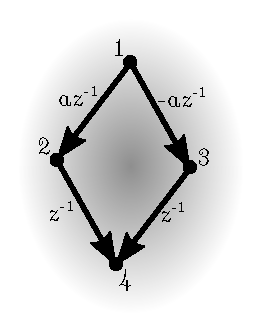
\includegraphics[width=\linewidth]{example1.pdf}
    \caption{Graph Corresponding to Example \ref{ex:diamond_cancellation}}
    \label{fig:diamond_cancellation}
    \centering{$j \in \anc{i} \nRightarrow j \pwgc i$}
  \end{subfigure}
  \begin{subfigure}[b]{0.45\textwidth}
    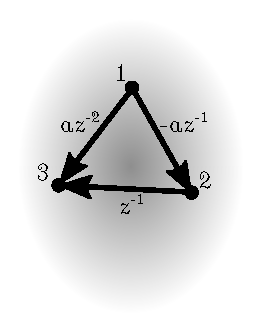
\includegraphics[width=\linewidth]{example2.pdf}
    \caption{Graph Corresponding to Example \ref{ex:lag_cancellation}}
    \label{fig:lag_cancellation}
    \centering{$j \in \pa{i} \nRightarrow j \pwgc i$}
  \end{subfigure}
\end{figure}

\begin{example}
  \label{ex:lag_cancellation}
  A second example on $n = 3$ nodes is also worth examining, in this case
  cancellation is a result of differing time lags.

\begin{equation*}
  x(t) =
  \left[
    \begin{array}{ccc}
      0 & 0 & 0\\
      -a & 0 & 0\\
      0 & 1 & 0\\
    \end{array}
  \right] x(t - 1) +
  \left[
    \begin{array}{ccc}
      0 & 0 & 0\\
      0 & 0 & 0\\
      a & 0 & 0\\
    \end{array}
  \right] x(t - 2) + v(t)
\end{equation*}

Then

\begin{align*}
  x_2(t) &= v_2(t) - ax_1(t - 1)\\
  x_3(t) &= v_3(t) + x_2(t - 1) + ax_1(t - 2)\\
  \Rightarrow x_3(t) &= v_2(t - 1) + v_3(t),
\end{align*}

and again $1 \npwgc 3$.
\end{example}

\subsection{Strongly Causal Graphs}
\label{sec:strongly_causal_graphs}
% The examples at the conclusion of the previous section seem rather
% pathological since we have simply constructed a case where different
% paths in the graph cancel exactly.  It may be possible to rid
% ourselves of these pathologies for instance by defining a notion of
% ``robust'' pairwise causality where ``$j \pwgc _R i$'' if $j \pwgc i$
% almost surely for a ``small'' random perturbation of the system
% matrix.  However, we do not believe such a modification of our theory
% can have useful practical implications since the difference between
% paths that ``nearly cancel'' rather than cancel exactly would in
% practice require inordinate amounts of data to resolve.

In this section and the next we will seek to understand when converse
statements of Proposition \ref{prop:ancestor_properties} \textit{do}
hold.  One possibility is to restrict the coefficients of the system
matrix, e.g. by requiring that $B_{ij}(\tau) \ge 0$.  Instead,
we think it more meaningful to focus on the defining feature of
time series networks, that is, the topology of $\gcg$.

\begin{definition}[Strongly Causal]
  \label{def:strongly_causal}
  We will say that a Granger-causality graph $\gcg$ is
  \textit{strongly causal} if there is at most 1 directed path between
  any two nodes.  Strongly Causal Graphs will be referred to as SCGs.
\end{definition}

Examples of strongly causal graphs include directed trees (or
forests), DAGs where each node has at most one parent, and figure
\ref{fig:example_fig3} of this paper.  A complete bipartite graph with
$2n$ nodes is also strongly causal, demonstrating that the number of
edges of such a graph can still scale quadratically with the number of
nodes.  It is evident that the strong causal property is inherited by
subgraphs.

\begin{example}
  Though examples of SCGs are easy to construct in theory, should
  practitioners expect SCGs to arise in application?  While a positive
  answer to this question is not \textit{necessary} for the concept to
  be useful, it is certainly sufficient.  Though the answer is likely
  to depend upon the particular application area, examples appear to
  be available in biology, in particular, the authors of
  \cite{discovering_graphical_Granger_causality_using_the_truncating_lasso_penalty}
  cite an example of the so called ``transcription regulatory network
  of \textit{E.coli}'', and
  \cite{learning_genome_scale_regulatory_networks} study a much larger
  regulatory network of \textit{Saccharomyces cerevisiae}.  These
  networks, which we reproduce\footnote{Figure \ref{fig:gene_network1}
    is reproduced under the Creative Commons Attribution
    Non-Commercial License
    (\url{http://creativecommons.org/licenses/by-nc/2.5}) and Figure
    \ref{fig:gene_network2} under the Creative Commons Attribution
    License (\url{https://creativecommons.org/licenses/by/4.0/})} in
  figure \ref{fig:gene_networks} appear to have at most a small number
  of edges which violate the strong-causality condition.

  \begin{figure}[h]
    \centering
    \caption{Transcription Regulatory Networks}
    \label{fig:gene_networks}
    \begin{subfigure}[b]{0.45\textwidth}
      \caption{\textit{E.Coli} Network of
        \cite{discovering_graphical_Granger_causality_using_the_truncating_lasso_penalty}}
      \label{fig:gene_network1}
      \includegraphics[width=\linewidth, height=\linewidth]{ecoli_regulatory_network.png}
    \end{subfigure}
    \begin{subfigure}[b]{0.45\textwidth}
      \caption{\textit{Saccharomyces cerevisiae} Network of
        \cite{learning_genome_scale_regulatory_networks}}
      \label{fig:gene_network2}
      \includegraphics[width=\linewidth, height=\linewidth]{huge_gene_network.png}
    \end{subfigure}
  \end{figure}
\end{example}

% \begin{lemma}
%   \label{lem:still_strongly_causal}
%   If $\gcg$ is a strongly causal graph, any subgraph formed by eliminating nodes
%   as well as all of the in and out edges thereof is still strongly causal.
% \end{lemma}
% \begin{proof}
%   If $\gcg$ has at most one path between any two nodes, there can only
%   be fewer paths after removing nodes from $\gcg$.
% \end{proof}

For later use, and to get a feel for the topological implications of
strong causality, we explore a number of properties of such graphs
before moving into the main result of this section.  The following
important property essentially strengthens proposition
\ref{prop:ancestor_properties} for the case of strongly causal graphs.

\begin{proposition}
  \label{prop:sc_graph_common_anc}
  In a strongly causal graph if $j \in \anc{i}$ then any
  $k \in \anc{i} \cap \anc{j}$ is not a confounder, that is,
  the unique path from $k$ to $i$ contains $j$.
\end{proposition}
\begin{proof}
  Suppose that there is a path from $k$ to $i$ which does not contain
  $j$.  In this case, there are multiple paths from $k$ to $i$ (one of
  which \textit{does} go through $j$ since $j \in \anc{i}$) which
  contradicts the assumption of strong causality.
\end{proof}

% Is pwgc transitive?
  
\begin{corollary}
  \label{cor:parent_corollary}
  If $\gcg$ is a strongly causal DAG then $i \pwgc j$ and $j \in \anc{i}$ are
  \textit{alternatives}, that is $i \pwgc j \Rightarrow j \notin \anc{i}$.
\end{corollary}
\begin{proof}
  Suppose that $i \pwgc j$ and $j \in \anc{i}$.  Then since $\gcg$ is
  acyclic $i \not\in \anc{j}$, and by proposition
  \ref{prop:ancestor_properties} there is some
  $k \in \anc{i}\cap\anc{j}$ which is a confounder.  However, by
  proposition \ref{prop:sc_graph_common_anc} $k$ cannot be a
  confounder, a contradiction.
\end{proof}
% This is a direct proof
  % \begin{proof}
%   Suppose that $\gcg$ is a strongly causal DAG and that we have both
%   $i \pwgc j$ and $j \in \anc{i}$, which implies that
%   $i \not \in \anc{j}$ since $\gcg$ is a DAG.  We will establish the
%   contradiction $i \in \anc{j}$.

%   Since $j \in \anc{i}$ there is a path $\gcgpath{j}{i}$.
%   Moreover, since $i \pwgc j$ by proposition \ref{prop:pwgc_anc} there
%   must be a confounding ancestor $k \in \anc{i} \cap \anc{j}$, where the
%   node $k$ has a path to $j,\ \gcgpath{k}{j}$, as well as a path
%   to $i,\ \gcgpath{k}{i}$.

%   \hl{Double check that the ancestor properties proposition implies
%     that BOTH paths do not contain the other node.}

%   Now, since the graph is strongly causal, the only possible
%   $\gcgpath{k}{i}$ path is the one obtained by concatenating the
%   $\gcgpath{k}{j}$ path with the $\gcgpath{j}{i}$ path.
%   However, this is a contradiction since $k$ is a confounder and
%   should have a $\gcgpath{k}{i}$ path which does not contain $i$.
% \end{proof}
  
\begin{corollary}
  \label{cor:bidirectional_edge}
  If $\gcg$ is a strongly causal DAG such that $i \pwgc j$ and
  $j \pwgc i$, then $i \not\in \anc{j}$ and $j \not\in \anc{i}$.  In
  particular, a pairwise bidirectional edge indicates the absence of
  any edge in $\gcg$.
\end{corollary}
\begin{proof}
  This follows directly from applying proposition
  \ref{cor:parent_corollary} to $i \pwgc j$ and $j \pwgc i$.
% This is a direct proof
% \begin{proof}
  % By way of contradiction, suppose that $i \in \pa{j}$.  We will
  % consider the two possibilities allowed by proposition
  % \ref{prop:ancestor_properties} for $j \pwgc i$.  Firstly
  % $j \in \anc{i}$ is impossible since $\gcg$ is assumed to be acyclic.
  % Secondly, if there is some confounding node
  % $u \in \anc{i} \cap \anc{j}$ with a path
  % $u \rightarrow \cdots \rightarrow j$ which does not contain $i$ we
  % have a contradiction since there must now be multiple
  % $u \rightarrow j$ paths: the aforementioned, and a path
  % $u \rightarrow \cdots \rightarrow i \rightarrow \cdots \rightarrow
  % j$ which \textit{does} contain $i$.  We conclude that $i \in \pa{j}$
  % is impossible, and symmetrically that $j \in \pa{i}$ is as well.
% \end{proof}
\end{proof}

% \begin{proposition}
%   \label{prop:independent_confounders}
%   If $\gcg$ is strongly causal we have distinct
%   $k_1, k_2 \in \anc{i} \cap \anc{j}$ are confounders of $i, j$, then
%   $k_1 \not\in \anc{k_2}$, $k_2 \not\in \anc{k_1}$ and
%   $\not\exists \ell \in \anc{k_1} \cap \anc{k_2}$ confounding
%   $k_1, k_2$.
% \end{proposition}
% \begin{proof}
%   \hl{TODO}
% \end{proof}

% \begin{corollary}
%   If $\gcg$ is strongly causal, then distinct confounders are
%   uncorrelated.
% \end{corollary}
% \begin{proof}
%   This follows directly by combining proposition
%   \ref{prop:independent_confounders} with proposition \ref{prop:ancestor_properties}.  \hl{I need to update prop} \ref{prop:ancestor_properties} \hl{to note the strong non-correlation property.}
% \end{proof}

% \begin{lemma}
%   If $\gcg$ is a strongly causal DAG and $j \in \anc{i}$ then 
% \end{lemma}

In light of proposition \ref{prop:sc_graph_common_anc}, the following
provides a partial converse to proposition
\ref{prop:ancestor_properties}, and supports the intuition of ``causal
flow'' through paths in $\gcg$.

\begin{proposition}
  \label{prop:pwgc_anc}
  If $\gcg$ is a strongly causal DAG then $j \in \anc{i} \Rightarrow j \pwgc i$.
\end{proposition}
\begin{proof}
  We will show that for some $\psi \in \H_{t - 1}^{(j)}$ we have

  \begin{equation}
    \label{eqn:cond_ortho_proof}
    \inner{\psi - \linE{\psi}{\H_{t - 1}^{(i)}}}{x_i(t) - \linE{x_i(t)}{\H_{t - 1}^{(i)}}} \ne 0
  \end{equation}

  and therefore that $H_t^{(i)} \not\perp\ \H_{t - 1}^{(j)}\ |\ \H_{t - 1}^{(i)}$, which by theorem (\ref{thm:granger_causality_equivalences}) is enough to establish that $j \pwgc i$.

  Firstly, we will establish a representation of $x_i(t)$ that involves $x_j(t)$.  Denote by $a_{r + 1} \rightarrow a_r \rightarrow \cdots \rightarrow a_1 \rightarrow a_0$ with $a_{r + 1} \defeq j$ and $a_0 \defeq i$ the \textit{unique} $\gcgpath{j}{i}$ path in $\gcg$, we will expand the representation of equation (\ref{eqn:parent_expansion}) backwards along this path:

  % Should this be written as a lemma?
  \begin{align*}
    x_i(t) &= v_i(t) + \B_{ii}(z) x_i(t) + \sum_{k \in \pa{i}}\B_{ik}(z) x_k(t)\\
           &= \underbrace{v_{a_0}(t) + \B_{a_0a_0}(z) x_i(t) + \sum_{\substack{k \in \pa{a_0} \\ k \ne a_1}}\B_{a_0 k}(z) x_k(t)}_{\defeq \wtalpha{a_0}{a_1}} + \B_{a_0a_1}(z)x_{a_1}(t)\\
           &= \wtalpha{a_0}{a_1} + \B_{a_0a_1}(z)\big[\wtalpha{a_1}{a_2} + \B_{a_1a_2}(z)x_{a_2}(t) \big]\\
           &\overset{(a)}{=} \sum_{\ell = 0}^r \underbrace{\Big(\prod_{m = 0}^{\ell - 1} \B_{a_m a_{m + 1}}(z) \Big)}_{\defeq F_\ell(z)} \wtalpha{a_\ell}{a_{\ell + 1}} + \Big(\prod_{m = 0}^{r}\B_{a_m a_{m + 1}}(z)\Big)x_{a_{r + 1}}(t)\\
           &= \sum_{\ell = 0}^r F_\ell(z) \wtalpha{a_\ell}{a_{\ell + 1}} + F_{r + 1}(z) x_j(t)
  \end{align*}

  where $(a)$ follows by a routine induction argument and where we define $\prod_{m = 0}^{-1} \bullet \defeq 1$ for notational convenience.

  Using this representation to expand equation (\ref{eqn:cond_ortho_proof}), we obtain the following cumbersome expression:

  \begin{align*}
    &\inner{\psi - \linE{\psi}{\H_{t - 1}^{(i)}}}{F_{r + 1}(z)x_j(t) - \linE{F_{r + 1}(z)x_j(t)}{\H_{t - 1}^{(i)}}}\\
    &- \inner{\psi - \linE{\psi}{\H_{t - 1}^{(i)}}}{\linE{\sum_{\ell = 0}^r F_\ell(z)\wtalpha{a_\ell}{a_{\ell + 1}}}{\H_{t - 1}^{(i)}}}\\
    &+ \inner{\psi - \linE{\psi}{\H_{t - 1}^{(i)}}}{\sum_{\ell = 0}^r F_\ell(z)\wtalpha{a_\ell}{a_{\ell + 1}}}.
  \end{align*}

  Note that by the orthogonality principle, $\psi - \linE{\psi}{\H_{t - 1}^{(i)}} \perp \H_{t - 1}^{(i)}$, the middle term above is $0$.  Choosing now the particular value $\psi = F_{r + 1}(z)x_j(t) \in \H_{t - 1}^{(j)}$ we arrive at

  \begin{align*}
    &\inner{\psi - \linE{\psi}{\H_{t - 1}^{(i)}}}{x_i(t) - \linE{x_i(t)}{\H_{t - 1}^{(i)}}}\\
    &= \E|F_{r + 1}(z)x_j(t) - \linE{F_{r + 1}(z)x_j(t)}{\H_{t - 1}^{(i)}}|^2\\
    &+ \inner{F_{r + 1}(z)x_j(t) - \linE{F_{r + 1}(z)x_j(t)}{\H_{t - 1}^{(i)}}}{\sum_{\ell = 0}^r F_\ell(z) \wtalpha{a_\ell}{a_{\ell + 1}}},
  \end{align*}

  which by the Cauchy-Schwarz inequality is $0$ if and only if

  \begin{equation*}
    \sum_{\ell = 0}^r F_\ell(z) \wtalpha{a_\ell}{a_{\ell + 1}} \overset{\text{a.s.}}{=} \linE{F_{r + 1}(z)x_j(t)}{\H_{t - 1}^{(i)}} - F_{r + 1}(z)x_j(t),
  \end{equation*}

  or by rearranging and applying the representation obtained earlier, if and only if

  \begin{equation*}
    x_i(t) \overset{\text{a.s.}}{=} \linE{F_{r + 1}(z)x_j(t)}{\H_{t - 1}^{(i)}},
  \end{equation*}

  but this is impossible since $x_i(t) \not \in \H_{t - 1}^{(i)}$.
\end{proof}

We immediately obtain the corollary, which we remind the reader is,
surprisingly, not true in a general graph.

\begin{corollary}
  \label{cor:gc_implies_pwgc}
  If $\gcg$ is a strongly causal DAG then $j \gc i \Rightarrow j \pwgc i$.
\end{corollary}

% \begin{remark}
%   It can be seen from the conclusion of the proof that simple facts
%   about Granger causality are indeed reliant on our assumptions about
%   the nature of $x(t)$ laid out in the section \ref{sec:theory}, in
%   particular, the innovations process $v(t)$ must be full rank.
  
%   Moreover, that strong conditions need to be placed on the topology
%   of $\gcg$ in order for proposition \ref{prop:pwgc_anc} to hold can
%   be seen through the earlier examples.
% \end{remark}

% This holds in any DAG
% \begin{lemma}
%   If $\gcg$ is strongly causal, then any $\\VAR(p)$ system on $\gcg$ is stable if and only if
%   $B_{ii}(z)$ is stable for every $i = 1, \ldots, n$.
% \end{lemma}
% \begin{proof}
%   \hl{This is certainly true, but I don't think I need to use it anywhere.}
% \end{proof}

\begin{remark}
  As we have seen and as is true in much of statistics, confounding
  nodes pose challenges for Granger-causality.  However, as opposed to
  Pearl's causal calculus \cite{pearl2000art}, pairwise
  Granger-causality does not suffer any difficulty with so-called
  ``colliders'', that is, the topology $i \rightarrow k \leftarrow j$
  will never result in $i \pwgc j$ or $j \pwgc i$.  This is evidently
  an advantage of the \textit{temporal} nature of Granger-causality -- there is
  no backwards causal flow along the edges of $\gcg$.
\end{remark}

\begin{example}
  As a final remark of this subsection we note that a complete
  converse to proposition \ref{prop:ancestor_properties} is not
  possible without additional conditions.  Consider the ``fork'' system on $3$
  nodes (i.e. $2 \leftarrow 1 \rightarrow 3$) defined by

  \begin{equation*}
    x(t) =
    \left[
      \begin{array}{cccc}
        0 & 0 & 0\\
        a & 0 & 0\\
        a & 0 & 0\\
      \end{array}
    \right] x(t - 1) + v(t).
  \end{equation*}

  In this case, node $1$ is a confounder for nodes $2$ and $3$, but
  $x_3(t) = v_3(t) - v_2(t) + x_2(t)$ and $2 \npwgc 3$ (even
  though $x_2(t)$ and $x_3(t)$ are contemporaneously correlated)

  If we were to augment this system by simply adding an autoregressive
  component (i.e. some ``memory'') to $x_1(t)$ e.g.
  $x_1(t) = v_1(t) + b x_1(t - 1)$ then we \textit{would} have
  $2 \pwgc 3$ since then
  $x_3(t) = v_3(t) + av_1(t - 1) - bv_2(t - 1) + bx_2(t - 1)$.  We
  develop this idea further in the next section.
\end{example}

\subsection{Persistent Systems}
\label{sec:persistent_systems}
In section \ref{sec:strongly_causal_graphs} we obtained a converse to
part $(a)$ of proposition \ref{prop:ancestor_properties} via the
notion of a strongly causal graph topology.  In this section, we
complete a converse by adding the additional requirement we refer to
as ``persistence''.

\begin{definition}[Lag Function]
  Given a causal filter $\B(z) = \sum_{\tau = 0}^\infty b(\tau)z^{-\tau}$
  define 

  \begin{align}
    \tau_0(\B) &= \text{min}\{\tau \in \Z_+\ |\ b(\tau) \ne 0\},\\
    \tau_{\infty}(\B) &= \text{sup}\{\tau \in \Z_+\ |\ b(\tau) \ne 0\}.\\
  \end{align}

  i.e. the ``first'' and ``last'' coefficients of the filter $\B(z)$,
  where $\tau_\infty(\B) \defeq \infty$ if the filter has an infinite
  length, and $\tau_0(\B) \defeq \infty$ if $\B(z) = 0$.
\end{definition}

This interpretation of the following persistence condition is that
each node stores some ``memory'' of the past.

\begin{definition}[Persistent]
  We will say that the process $x(t)$ with Granger-causality graph
  $\gcg$ is \textit{persistent} if for every $i \in [n]$ and every
  $k \in \anc{i}$ we have $\tau_0(\A_{ik}) < \infty$ and $\tau_\infty(\A_{ik}) = \infty$.
\end{definition}

\begin{remark}
  In the context of Granger-causality, ``most'' systems should be
  persistent.  In particular, $\mathsf{\VAR}(p)$ models are likely to
  be persistent since these naturally result in an equivalent
  $\mathsf{MA}(\infty)$ representation, except for the pathological
  case where $\B(z)$ is Nilpotent.

  Moreover, persistence is not the weakest condition necessary for the
  results of this section, the condition
  $\tau_0(\A_{jk}) < \tau_\infty(\A_{ik})$ for each $i, j, k$ such that
  $k \in \anc{i} \cap \anc{j}$ is enough.  The intuition being that nodes
  $i$ and $j$ are not receiving temporally disjoint information from
  $k$.

\end{remark}

\begin{example}
  process $x(t)$ generated by the $\VAR(1)$ model\footnote{Recall that
    any $\VAR(p)$ model with $p < \infty$ can be written as a
    $\VAR(1)$ model, so we lose little generality in considering this
    case.}  having $\B(z) = Bz^{-1}$, we will examine
  conditions that guarantee persistence.  Pick any
  $i \in [n], j \in \anc{i} \setminus \{i\}$, then the stability of
  $B$ allows us to write

  \begin{equation*}
    \A(z) = \sum_{k = 0}^\infty B^k z^{-k},
  \end{equation*}

  whereby we see that $\exists k > 0$ such that $[B^k]_{ij} \ne 0$
  (since $j \in \anc{i}$).  Then consider

  \begin{equation*}
    \begin{aligned}
      e_i^\T B^{rk} e_j &\overset{(a)}{=} \big((P^\T e_i)^\T J^{rk} P^{-1}e_j\big)\\
      &= \tr [(P^\T e_i)^\T J^{rk} P^{-1}e_j]\\
      &\overset{(b)}{=} \tr [(J^{rk}) (v u^\T)],
    \end{aligned}
  \end{equation*}

  where $(a)$ utilizes the Jordan Normal Form of $B$, and $(b)$
  denotes $u = P^\T e_i$ and $v = P^{-1}e_j$.  In order for
  $\tau_\infty(\A_{ij}) < \infty$, there must be some $N > 1$ such
  that $\forall r \ge N$, the above term is $0$.  This may be the case
  for instance if $B$ is a nilpotent matrix.  

  Let us suppose now that $B$ is diagonalizable (i.e. $J$ is a
  diagonal matrix) with at least $2$ distinct eigenvalues; in this
  case $B$ is also \textit{not} nilpotent.  We can then rewrite the
  above as

  \begin{equation*}
    f(r) \defeq \tr [(J^{rk}) (v u^\T)] = \sum_{\nu = 1}^n \lambda_\nu ^{rk} v_\nu u_\nu \defeq \sum_{\nu = 1}^n \lambda_\nu^{rk} \beta_\nu
  \end{equation*}

  where $\lambda_\nu$ denotes the eigenvalues of $B$ and
  $\beta_\nu = u_\nu v_\nu$.  Note that $f(0) = 0$ since $i \ne j$,
  $u$ is a row of $P$ and $v$ is a column of $P^{-1}$.  Moreover,
  $f(1) \ne 0$ by hypothesis.  But, in order for
  $f(r) = 0\ \forall r \ge N$, it would need to be the case that

  \begin{equation*}
    \Dg(\bm{\lambda})^r \bm{\lambda} = Vz
  \end{equation*}

  had a solution in $z$ for every $r \ge N$, where $V$ is an
  $n \times n - 1$ full-rank matrix whose columns span the nullspace of $\beta$,
  and $\bm{\lambda} = (\lambda_1, \ldots, \lambda_n)$. That is,
  iterates of $\Dg(\bm{\lambda})$ applied to $\bm{\lambda}$ would need to remain
  inside $\beta$'s nullspace.  This would imply that

  \begin{equation*}
    VV^\dagger \bm{\lambda}^{r + 1} = \bm{\lambda}^{r + 1},
  \end{equation*}

  i.e. that $\bm{\lambda}^{r + 1}$ is an eigenvector of $VV^\dagger$
  for an infinite number of integers $r$ (the exponentiation is to be
  understood as a pointwise operation).  However, since there can only
  be a finite number of (unit length) eigenvectors, this cannot be the
  case unless every eigenvalue $(\lambda_1, \ldots, \lambda_n)$ were
  equal.

  We see from this example that the collection of $\VAR(1)$ systems
  which are not persistent are pathological, in the sense that their
  system matrices have zero measure when viewed as a subset of $\R^{n^2}$.
\end{example}

\begin{lemma}
  \label{lem:time_lag_cancellation}
  Suppose $v(t)$ is a scalar sequence with unit variance and zero
  autocorrelation and let $\A(z), \B(z)$ be nonzero and strictly
  causal (i.e. $\tau_0(\A) \ge 1$) linear filters.  Then,

  \begin{equation}
    \inner{F(z)\A(z)v(t)}{\B(z)v(t)} = 0\ \forall \text{ strictly causal filters } F(z)
  \end{equation}

  if and only if $\tau_0(\A) \ge \tau_\infty(\B)$.
\end{lemma}
\begin{proof}
  We have

  \begin{align}
    \inner{\A(z)v(t)}{\B(z)v(t)} &= \sum_{\tau = 1}^\infty \sum_{s = 1}^\infty a(\tau)b(s)\E[v(t - s)v(t - \tau)]\\
    &= \sum_{\tau = \text{max}(\tau_0(\A), \tau_0(\B))}^{\text{min}(\tau_\infty(\A), \tau_\infty(\B))} a(\tau) b(\tau)\\
  \end{align}

  due to the uncorrelatedness assumptions on $v(t)$.  This expression
  is $0$ if and only if $\tau_0(\A) \ge 1 + \tau_\infty(\B)$ or if
  $\tau_0(\B) \ge 1 + \tau_\infty(\A)$ or if the coefficients are
  orthogonal along the common support.

  Specializing this fact to $\inner{F(z)\A(z)v(t)}{\B(z)v(t)} = 0$ we
  see that the coefficients cannot be orthogonal for every choice of
  $F$, and that $\text{sup}_F \tau_\infty(F\A) = \infty$, leaving only
  the possibility that

  \begin{align*}
    \tau_0(F\A) \ge 1 + \tau_\infty(\B) \forall F &\overset{(a)}{\iff} \tau_0(\A) \ge 1 + \tau_\infty(\B) - \underset{F}{\text{min }} \tau_0(F)\\
    &\overset{(b)}{\iff} \tau_0(\A) \ge \tau_\infty(\B),
  \end{align*}

  where $(a)$ follows since $\tau_0(F\A) = \tau_0(F) + \tau_0(\A)$,
  and $(b)$ since $\text{min}_F\ \tau_0(F) = 1$.
\end{proof}

\begin{corollary}
  \label{cor:time_lag_cancellation}
  For $k \in \anc{i} \cap \anc{j}$ we have

  \begin{align*}
    \linE{F(z)\A_{jk}(z)v_k(t)}{\H_{t - 1}^{(i)}} &= 0\ \forall \text{ strictly causal } F(z)\\
    \iff \inner{F(z)\A_{jk}(z)v_k(t)}{\A_{ik}(z)v_k(t)} &= 0\ \forall \text{ strictly causal } F(z)\\
    \iff \tau_0(\A_{jk}) \ge \tau_\infty(\A_{ik})
  \end{align*}
\end{corollary}
\begin{proof}
  The final equivalence follows immediately from Lemma \ref{lem:time_lag_cancellation}.  For the first equivalence we have

  \begin{align*}
    \linE{F(z)\A_{jk}(z)v_k(t)}{\H_{t - 1}^{(i)}} &= 0\ \forall \text{ strictly causal } F(z)\\
    \iff \inner{F(z)A_{jk}(z)v_k(t)}{x_i(t - \tau)} &= 0\ \forall \tau \ge 1, \text{ strictly causal } F(z),
  \end{align*}

  which can be expanded by equation \eqref{eqn:ancestor_expansion} to
  obtain (after cancelling all ancestors of $i$ other than $k$)

  \begin{equation*}
    \inner{F(z)A_{jk}(z)v_k(t)}{\A_{ik}(z)v_k(t - \tau)} = 0\ \forall \tau \ge 1, \text{ strictly causal } F(z),
  \end{equation*}

  which by the Lemma is equivalent to $\tau_0(\A_{jk}) \ge \tau_\infty(\A_{ik})$ as stated.
\end{proof}

\begin{proposition}
  \label{prop:persistence_converse}
  Suppose $\gcg$ is a strongly causal DAG and that $x(t)$ is
  persistent, then if there exists a $k$ which confounds $(i, j)$ we
  have $i \pwgc j$ and $j \pwgc i$.
\end{proposition}
\begin{proof}
  We will show that $j \pwgc i$, the other being symmetric.  First
  note also that by proposition \ref{prop:sc_graph_common_anc} we
  cannot have $i \in \anc{j}$ or $j \in \anc{i}$ and therefore every
  $k \in \anc{i}\cap\anc{j}$ will be a confounder.

  It is sufficient to show that $\exists \psi \in \H_{t - 1}^{(j)}$
  such that

  \begin{equation*}
    \inner{\psi - \linE{\psi}{\H_{t - 1}^{(i)}}}{x_i(t) - \linE{x_i(t)}{\H_{t - 1}^{(i)}}} \ne 0.
  \end{equation*}

  To this end, let $F(z)$ be an arbitrary but strictly causal linear
  filter.  We apply equation \eqref{eqn:ancestor_expansion} to
  $x_i(t)$ and $\psi \defeq F(z)x_j(t)$:

  \begin{align*}
    &\inner{\psi - \linE{\psi}{\H_{t - 1}^{(i)}}}{x_i(t) - \linE{x_i(t)}{\H_{t - 1}^{(i)}}}\\
    &\overset{(a)}{=} \inner{\psi - \linE{\psi}{\H_{t - 1}^{(i)}}}{\A_{ii}(z)v_i(t) + \sum_{k \in \anc{i}}\A_{ik}(z)v_k(t)}\\
    &\overset{(b)}{=} \inner{\sum_{k \in \anc{j}}\big(F(z)\A_{jk}(z)v_k(t) - \linE{F(z)\A_{jk}(z)v_k(t)}{\H_{t - 1}^{(i)}}\big)}{\A_{ii}(z)v_i(t) + \sum_{k \in \anc{i}}\A_{ik}(z)v_k(t)}\\
    &\overset{(c)}{=} \sum_{k \in \anc{i}\cap\anc{j}}\Big(\inner{F(z)\A_{jk}(z)v_k(t)}{\A_{ik}(z)v_k(t)} - \inner{\linE{F(z)\A_{jk}(z)v_k(t)}{\H_{t - 1}^{(i)}}}{\A_{ii}v_i(t)}\\
    &- \sum_{\ell \in \anc{i}}\inner{\linE{F(z)\A_{jk}(z)v_k(t)}{\H_{t - 1}^{(i)}}}{\A_{i\ell}(z)v_\ell(t)}\Big)
  \end{align*}

  where in $(a)$ we have removed the $\linE{x_i(t)}{\H_{t - 1}^{(i)}}$
  term via the orthogonality principle, in $(b)$ there is no
  $F(z)\A_{jj}(z)v_j(t)$ term since due to $j \not\in \anc{i}$ it is
  orthogonal to $\H_t^{(i)}$.  Finally, $(c)$ follows by applying
  orthogonality properties of $v(t)$, as well as the fact that
  $\linE{F(z)\A_{jk}(z)v_k(t)}{\H_{t - 1}^{(i)}} = 0$ for
  $k \not \in \anc{i}$.  Note that
  $\linE{F(z)\A_{jk}(z)v_k(t)}{\H_{t - 1}^{(i)}} \in \H_{t - 1}^{(i)}$
  and thence there is in general no cancellation in the final term
  above for $\ell \in \anc{i}$.

  \todo{This is clearly not immediately evident}

  This is $0$ for every $F$ if and only if for all $F$ and
  $\forall k \in \anc{i} \cap \anc{j}$ we have
  $$\linE{F(z)\A_{jk}(z)v_k(t)}{\H_{t - 1}^{(i)}} = 0$$ and
  $$\inner{F(z)\A_{jk}(z)v_k(t)}{\A_{ik}(z)v_k(t)} = 0,$$ which by
  Corollary \ref{cor:time_lag_cancellation} occurs if and only if
  $\tau_0(\A_{jk}) \ge \tau_\infty(\A_{ik})$, which is impossible since by persistence
  $\tau_0(\A_{jk}) < \infty$ and  $\tau_\infty(\A_{ik}) = \infty$.
\end{proof}

\subsection{Recovering $\gcg$ via Pairwise Tests}
\label{sec:pairwise_algorithm}
In this section we will show that if the $\gcg$ of a persistent
process is a strongly causal DAG, then it is possible to recover
$\gcg$ via pairwise tests alone.  This is the main conclusion of the
theoretical analysis in this paper.

% This is an interesting fact in and
% of itself, but also has some implications for applications since
% pairwise testing is trivially parallelizable.  In section
% \ref{sec:structure_learning} we will also analyze the use of pairwise
% testing as a heuristic for general graphs.

\begin{theorem}[Pairwise Recovery]
  \label{thm:scg_recovery}
  If the Granger-causality graph $\gcg$ for persistent process $x(t)$
  is a strongly causal DAG then $\gcg$ can be inferred from pairwise
  causality tests.  The procedure can be carried out, assuming
  we have an oracle for pairwise causality, via Algorithm
  (\ref{alg:pwgr}).

  \begin{algorithm}
    \SetKwInOut{Input}{input}
    \SetKwInOut{Output}{output}
    \SetKwInOut{Initialize}{initialize}
    \DontPrintSemicolon

    \BlankLine
    \caption{Pairwise Graph Recovery}
    \label{alg:pwgr}
    % \TitleOfAlgo{Pairwise Graph Recovery}
    \Input{Pairwise Granger-causality relations between a persistent
      process of dimension $n$ whose joint Granger-causality
      relations are known to form a strongly causal DAG $\gcg$.}
    \Output{Edges $\gcge = \{(i, j) \in [n] \times [n]\ |\ i \gc j \}$ of
      the graph $\gcg$.}
    \Initialize{$S_0 = [n]$  \texttt{\# unprocessed nodes}\\
      $E_0 = \emptyset$  \texttt{\# edges of }$\gcg$\\
      % $P_0 = \emptyset$  \texttt{\# layer by layer driving nodes}\\
      $k = 1$ \texttt{\# a counter used only for notation}}
    \BlankLine
    $W \leftarrow \{(i, j)\ |\ i \pwgc j, j \npwgc i\}$  \texttt{\# candidate edges}\\
    $P_0 \leftarrow \{i \in S_0\ |\ \forall s \in S_0\ (s, i) \not\in W\}$  \texttt{\# parent-less nodes}\\
    \While{$S_{k - 1} \ne \emptyset$}{
      $S_k \leftarrow S_{k - 1} \setminus P_{k - 1}$ \texttt{\# remove nodes with depth }$k - 1$\\
      $P_k \leftarrow \{i \in S_k\ |\ \forall s \in S_k\ (s, i) \not\in W\}$   \texttt{\# candidate children of }$P_{k - 1}$\\
      \;

      $D_{k0} \leftarrow \emptyset$\\
      \For{$r = 1, \ldots, k$} 
      {
        $Q \leftarrow E_{k - 1} \cup \big(\bigcup_{\ell = 0}^{r - 1} D_{k\ell}\big)$ \texttt{\# currently known edges}\\
        $D_{kr} \leftarrow \{(i, j) \in P_{k - r} \times P_k\ |\ (i, j) \in W,\ \text{no } \gcgpath{i}{j} \text{ path in } Q\}$
        % $E_k \leftarrow E_{k - 1} \cup D_{kr}$ \texttt{\# add edges to }$E_k$ \label{alg:inner_loop_end}\\
        % $W_{k + 1} \leftarrow W_k \setminus D_{kr}$  \texttt{\# remove edges from consideration}\\
      }
      $E_k \leftarrow E_{k - 1} \cup \big(\bigcup_{r = 1}^k D_{kr}\big)$ \texttt{\# update } $E_k$ \texttt{ with new edges}\\
      % \label{alg_line:inner_loop_end}\\
      % $W_{k + 1} \leftarrow W_k \setminus \big(\bigcup_{r = 0}^k D_{kr}\big)$  \texttt{\# remove edges from consideration}\\
      \;
      $k \leftarrow k + 1$
    }
    \Return{$E_{k - 1}$}
  \end{algorithm}
\end{theorem}

We will shortly prove the theorem by establishing the correctness of
algorithm (\ref{alg:pwgr}).  The idea is to iteratively ``peel away
layers'' of nodes by removing the nodes that have no parents
remaining, which always exist since the graph is acyclic.  The
requirement of strong causality ensures that all actual edges of
$\gcg$ manifest in some way as pairwise relations (by proposition
\ref{prop:pwgc_anc}), and the requirement of persistence allows
confounding to be eliminated by removing bidirectional edges.  Without
persistence, each confounded pair would give rise to $4$ possible
pairwise topologies consistent with $\gcg$, one for each type of
pairwise edge (no edge, unidirectional, bidirectional).

\begin{example}
  The set $W$ collects ancestor relations in $\gcg$ (see Lemma
  \ref{lem:W_subset_E}).  In reference to figure
  \ref{fig:example_fig3}, each of the solid black edges, as well as
  the dotted red edges will be included in $W$, but \textit{not} the
  bidirectional green dash-dotted edges, which we are able to exclude
  by appealing to Corollary \ref{cor:bidirectional_edge}.  The
  groupings $P_0, \ldots, P_3$ are also indicated in figure
  \ref{fig:example_fig3}.

  The algorithm proceeds first with the parentless nodes $1, 2$ on the
  initial iteration where the edge $(1, 3)$ is added to $E$.  On the
  next iteration, the edges $(3, 4), (2, 4), (3, 5)$ are added, and
  the false edges $(1, 4), (1, 5)$ are excluded due to the paths
  $1 \rightarrow 3 \rightarrow 4$ and $1 \rightarrow 3 \rightarrow 5$
  already being present.  Finally, edge $(4, 6)$ is added, and the false
  $(1, 6), (3, 6), (2, 6)$ edges are similarly excluded due to the
  ordering of the inner loop.
  
  \begin{figure}
    \centering
    \caption{Example graph for Algorithm \ref{alg:pwgr}}
    \footnotesize{Black arrows indicate true parent-child
      relations.  Red dotted arrows indicate pairwise causality (due to
      non-parent relations), green dash-dotted arrows indicate
      bidirectional pairwise causality (due to the confounding node
      $1$).  Blue groupings indicate each $P_k$ in Algorithm
      \ref{alg:pwgr}.}
    \label{fig:example_fig3}
    
    \begin{subfigure}[b]{0.45\textwidth}
      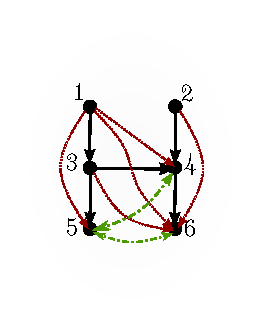
\includegraphics[width=\linewidth]{example_algorithm.pdf}
    \end{subfigure}
    \begin{subfigure}[b]{0.45\textwidth}
      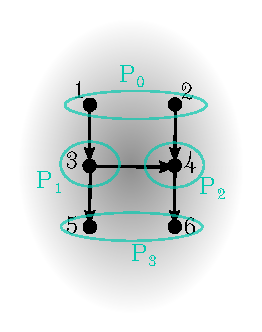
\includegraphics[width=\linewidth]{example_algorithm2.pdf}
    \end{subfigure}
  \end{figure}

  That we need to proceed backwards through $P_{k - r}$ as in the
  inner loop of on $r$ can also be seen from this example, where if
  instead we simply added the set

  \begin{equation*}
    D_k' = \{(i, j) \in \Big(\bigcup_{r = 1}^k P_{k - r}\Big) \times P_k\ |\ i \pwgc j \}
  \end{equation*}

  to $E_k$ then we would infer the false positive edge
  $1 \rightarrow 4$.  Moreover, the same example shows that simply
  using the set

  \begin{equation*}
    D_k'' = \{(i, j) \in P_{k - 1} \times P_k\ |\ i \pwgc j \}  ,
  \end{equation*}

  causes the edge $1 \rightarrow 3$ to be missed.
\end{example}

% \begin{lemma}
%   \label{lem:inner_loop_lemma}
%   At any given iteration, $k$, of Algorithm \ref{alg:pwgr}, if we have
%   $e \in E$ if and only if $e \in \gcge$, then the inner loop (line \ref{alg:inner_loop})
%   will add $(i, j) \in \big(\bigcup_{r = 0}^kP_{k - r}\big) \times C_k$ to $E$
%   if $(i, j) \in \gcge$.  i.e. any real edge will be included.
% \end{lemma}
% \begin{proof}
%   Let $j \in C_k$, $i \in \bigcup_{r = 0}^k P_{k - r}$, and assume
%   $i \in \pa{j}$.

%   First, suppose that there is no $i \rightarrow j$ path in $E$.  Then
%   since $i \gc j$ we have $i \pwgc j$ and $j \npwgc i$ (i.e.
%   $(i, j) \in W$) by Proposition \ref{prop:pwgc_anc} and Corollary
%   \ref{cor:bidirectional_edge} so at least one of
%   $\{D_{kr} \}_{r = 0}^k$ contains $(i, j)$ and hence $(i, j)$ will be
%   added to $E$ upon the end of the iteration.

%   Now, suppose instead that there is already an $i \rightarrow j$ path
%   in $E$.  Given our assumption that $E$ contains edges if and only if
%   they are edges of $\gcg$, then either we already have $(i, j) \in E$
%   correctly, or there is more than one $i \rightarrow j$ path in
%   $\gcg$, which is not possible since $\gcg$ is strongly causal.
% \end{proof}

% \begin{lemma}
%   \label{lem:W_subset_E}
%   $W \subseteq \gcge$
% \end{lemma}
% \begin{proof}
%   By proposition \ref{prop:pwgc_anc} we have
%   $j \in \pa{i} \Rightarrow j \pwgc i$ and by Corollary \ref{cor:bidirectional_edge}
%   there are no bidirectional edges in $\gcg$.
% \end{proof}

% \hl{Must show that Algorithm terminates in $n$ steps.}
% \begin{lemma}
%   For any $i \in P_k$ we have $i \in C_{k - 1}$.  \hl{[Can't yet prove
%     this part] Moreover, for each $i \in \bigcup_{k = 0}^n P_k$, if
%     $(s, i) \in W$ then $(s, i) \in E$ upon the termination of
%     Algorithm} \ref{alg:pwgr}.
% \end{lemma}
% \begin{proof}
%   We prove the second part by induction, the first part being
%   established along the way.  By construction $P_0$ has no parent
%   nodes in $\gcg$ so the base case is immediate.  Fix now some
%   $k \ge 1$, $i \in P_k$, and let $s$ be such that $(s, i) \in W$.
%   For every $s$ such that $(s, i) \in W$ we have $s \not\in S_k$ since
%   otherwise $i \not\in P_k$.  Therefore
%   $s \in \bigcup_{r = 0}^{k - 1}P_{k - r}$, which implies
%   $s \not\in S_k$, and finally that $i \in C_{k - 1}$.  Then by Lemma
%   \ref{lem:W_subset_E} every edge in $\gcge$ is also present in
%   $W$, and by Lemma \ref{lem:inner_loop_lemma} \hl{[We can't conclude
%     here because of the strong conditions required on lemma}
%     \ref{lem:inner_loop_lemma}]
% \end{proof}

% \begin{lemma}[Loop Invariant]
%   \label{lem:loop_invariant}
%   $\forall k \ge 0,\ e \in E_k \Rightarrow e \in \gcge$.
%   \hl{Not sure if this is useful / the right approach.}
% \end{lemma}
% \begin{proof}
%   We will proceed by induction.  Firstly, the base case
%   $E_0 = \emptyset$ is trivial, so fix some $k \ge 1$ and consider an
%   edge $(i, j) \in \big(\bigcup_{r = 0}^k P_{k - r} \big) \times C_k$
%   such that $(i, j) \in W$ (if the edge is not in $W$ then it is not
%   in $\gcge$ by Lemma \ref{lem:W_subset_E}).

%   \hl{WIP}
% \end{proof}

Our proof proceeds in 5 steps stated formally as lemmas.  Firstly, we
characterize the sets $W$ and $P_k$.  Then we establish a correctness
result for the inner loop on $r$, a correctness result for the outer
loop on $k$, and finally that the algorithm terminates in a finite
number of steps.

\begin{lemma}[$W$ Represents Ancestor Relations]
  \label{lem:W_subset_E}
  In Algorithm \ref{alg:pwgr} we have
  $(i, j) \in W$ if and only if $i \in \anc{j}$.  In particular,
  $W \subseteq \gcge$.
\end{lemma}
\begin{proof}
  Let $j \in [n]$ and suppose that $i \in \anc{j}$.  Then $i \pwgc j$
  by Proposition \ref{prop:pwgc_anc}.  Proposition
  \ref{prop:sc_graph_common_anc} ensures that $(i, j)$ are not
  confounded and Corollary \ref{cor:parent_corollary} that
  $j \not\in \anc{i}$ so $j \npwgc i$ and thence by Proposition
  \ref{prop:ancestor_properties} $(i, j) \in W$.

  Conversely, suppose $(i, j) \in W$.  Then since $j \npwgc i$
  Proposition \ref{prop:persistence_converse} ensures that $(j, i)$
  are not confounded and so by Proposition \ref{prop:ancestor_properties}
  we must have $i \in \anc{j}$.
\end{proof}

\begin{definition}[Depth]
  For our present purposes we will define the \textit{depth} $d(j)$ of
  a node $j$ in $\gcg$ to be the length of the \textit{longest} path
  from a node in $P_0$ to $j$, where $d(j) = 0$ if $j \in P_0$.  It is
  apparent that such a path will always exist.  For example, in Figure
  \ref{fig:example_fig3} we have $d(3) = 1$ and $d(4) = 2$.
\end{definition}

\begin{lemma}[Depth Characterization of $P_k$]
  \label{lem:depth_lemma}
  $i \in P_k \iff d(i) = k$ and $j \in S_k \iff d(j) \ge k$.
\end{lemma}
\begin{proof}
  We proceed by induction, noting that $P_0$ is non-empty since $\gcg$
  is acyclic and therefore $\gcg$ contains nodes without parents.  The
  base case $i \in P_0 \iff d(i) = 0$ is by definition, and
  $j \in S_0 \iff d(j) \ge 0$ is trivial since $S_0 = [n]$.  So
  suppose that the lemma is true up to $k - 1$.

  ($i \in P_k \implies d(i) = k$): Let $i \in P_k$.  Suppose that
  $d(i) \ge k + 1$, then $\exists j \in \pa{i}$ such that
  $j \not\in \cup_{r \ge 1}P_{k - r}$ (otherwise $d(i) \le k$), this
  implies that $j \in S_k$ with $(j, i) \in W$ (by Lemma
  \ref{lem:W_subset_E}) which is not possible due to the construction of
  $P_k$ and therefore $d(i) \le k$.  Moreover,
  $P_k \subseteq S_k \subseteq S_{k - 1}$ implies that
  $d(i) \ge k - 1$ by the induction hypothesis, but if $d(i) = k - 1$
  then $i \in P_{k - 1}$ again by induction which is impossible since
  $i \in P_k$ and therefore $d(i) = k$.

  ($s \in S_k \implies d(s) \ge k$): Let
  $s \in S_k \subseteq S_{k - 1}$.  We have by induction that
  $d(s) \ge k - 1$, but again by induction (this time on $P_{k - 1}$)
  we have $d(s) \ne k - 1$ since $S_k = S_{k - 1} \setminus P_{k - 1}$
  and therefore $d(s) \ge k$.

  ($d(i) = k \implies i \in P_k$): Suppose $i \in [n]$ is such that
  $d(i) = k$.  Then $i \in S_{k - 1}$ by the hypothesis, but also
  $i \not\in P_{k - 1}$ so then
  $i \in S_k = S_{k - 1} \setminus P_{k - 1}$ and thus $d(i) \ge k$.
  Now, recalling the definition of $P_k$

  \begin{equation*}
    P_k = \{i \in S_k\ |\ \forall s \in S_k\ (s, i) \not\in W \},
  \end{equation*}

  if $s \in S_k$ is such that $(s, i) \in W$ then $s \pwgc i$ and
  $i \npwgc s$ so that by persistence and Proposition
  \ref{prop:persistence_converse} there cannot be a confounder of
  $(s, i)$ (otherwise $i \pwgc s$) so then by Proposition
  \ref{prop:ancestor_properties} we have $s \in \anc{i}$.  We have
  shown that $s \in S_k \implies d(s) \ge k$ and so we must have
  $d(i) > k$, a contradiction, thence $s \not\in \anc{i}$,
  $s \npwgc i$, $(s, i) \not\in W$ and $i \in P_k$.

  ($d(j) \ge k \implies j \in S_k$): Let $j \in [n]$ such that
  $d(j) \ge k$, then by induction we have $j \in S_{k - 1}$.  This
  implies by the construction of $S_k$ that $j \not\in S_k$ only if
  $j \in P_{k - 1}$, but we have shown that this only occurs when
  $d(j) = k - 1$, but $d(j) > k - 1$ so $j \in S_k$.
\end{proof}

\begin{lemma}[Inner Loop]
  \label{lem:inner_loop_lemma}
  Fix an integer $k \ge 1$ and suppose that $(i, j) \in E_{k - 1}$ if
  and only if $(i, j) \in \gcge$ and $d(j) \le k - 1$.  Then, we have
  $(i, j) \in D_{kr}$ if and only if $(i, j) \in \gcge $, $d(j) = k$,
  and $d(i) = k - r$.
\end{lemma}
\begin{proof}
  We prove by induction on $r$, keeping in mind the results of Lemmas
  \ref{lem:W_subset_E} and \ref{lem:depth_lemma}.  For the base case,
  let $r = 1$ and suppose that $(i, j) \in \gcge$ with $d(j) = k$ and
  $d(i) = k - 1$.  Then, $(i, j) \in W$ and by our assumptions on
  $E_{k - 1}$ there is no $\gcgpath{i}{j}$ path in $E_{k - 1}$
  and therefore $(i, j) \in D_{k1}$.  Conversely, suppose that
  $(i, j) \in D_{k1}$.  Then, $d(i) = k - 1$ and $d(j) = k$ which, since
  $(i, j) \in W \implies i \in \anc{j}$ implies that
  $i \in \pa{j}$ and $(i, j) \in \gcge$.

  Now, fix $r > 1$ and suppose that the result holds up to $r - 1$.
  Let $(i, j) \in \gcge$ with $d(j) = k$ and $d(i) = k - r$.  Then,
  $(i, j) \in W$ and by induction and strong causality there cannot
  already be an $\gcgpath{i}{j}$ path in
  $E_{k - 1} \cup \big(\bigcup_{\ell = 0}^{r - 1} D_{kr}\big)$,
  therefore $(i, j) \in D_{kr}$.  Conversely, suppose
  $(i, j) \in D_{kr}$.  Then we have $d(i) = k - r$, $d(j) = k$, and
  $i \in \anc{j}$.  Suppose by way of contradiction that
  $i \not\in \pa{j}$, then there must be some $u \in \pa{j}$ such that
  $i \in \anc{u}$.  But, this implies that $d(i) < d(u)$ and by
  induction that $(u, j) \in \bigcup_{\ell = 1}^{r - 1}D_{k\ell}$.
  Moreover, since $d(u) < k$ (otherwise $d(j) > k$) each edge in
  the $\gcgpath{i}{u}$ path must already be in $E_{k - 1}$, and so
  there must be an $\gcgpath{i}{j}$ path in
  $E_{k - 1}\cup\big(\bigcup_{\ell = 0}^{r - 1}D_{kr}\big)$, which is
  a contradiction since we assumed $(i, j) \in D_{kr}$.  Therefore
  $i \in \pa{j}$ and $(i, j) \in \gcge$.
\end{proof}

\begin{lemma}[Outer Loop]
  \label{lem:outer_loop_lemma}
  We have $(i, j) \in E_k$ if and only if $(i, j) \in \gcge$ and
  $d(j) \le k$.  That is, at iteration $k, E_k$ and $\gcge$ agree on
  the set of edges whose terminating node is at most $k$ steps away
  from $P_0$.
\end{lemma}
\begin{proof}
  We will proceed by induction.  The base case $E_0 = \emptyset$ is
  trivial, so fix some $k \ge 1$, and suppose that the lemma holds for
  all nodes of depth less than $k$.

  Suppose that
  $(i, j) \in E_k = E_{k - 1}\cup \big(\bigcup_{r = 1}^k D_{rk}
  \big)$.  Then clearly there is some $1 \le r \le k$ such that
  $(i, j) \in D_{kr}$ so that by Lemma \ref{lem:inner_loop_lemma} we
  have $(i, j) \in \gcge$ and $d(j) = k$.

  Conversely, suppose that $(i, j) \in \gcge$ and $d(j) \le k$.  If
  $d(j) < k$ then by induction $(i, j) \in E_{k - 1} \subseteq E_k$ so
  suppose further than $d(j) = k$.  Since $i \in \pa{j}$ we must have
  $d(i) < k$ (else $d(j) > k$) and again by Lemma
  \ref{lem:inner_loop_lemma} $(i, j) \in \bigcup_{r = 1}^k D_{kr}$
  which implies that $(i, j) \in E_k$.  The result follows.
\end{proof}

\begin{lemma}[Finite Termination]
  Algorithm \ref{alg:pwgr} terminates and returns $E_{k^\star - 1} = \gcge$
  for some $k^\star \le n$.
\end{lemma}
\begin{proof}
  If $n = 1$, the algorithm is clearly correct, returning on the first
  iteration with $E_1 = \emptyset$.  When $n > 1$ Lemma
  \ref{lem:outer_loop_lemma} ensures that $E_k$ coincides with
  $\{(i, j) \in \gcge\ |\ d(j) \le k\}$ and since $d(j) \le n - 1$ for
  any $j \in [n]$ there is some $k^\star \le n$ such that
  $E_{k^\star - 1} = \gcge$.  We must have $S_{k^\star} = \emptyset$
  since $j \in S_{k^\star} \iff d(j) \ge k^\star$ (if $d(j) > k - 1$ then
  $E_{k^\star - 1} \ne \gcge$) and therefore the algorithm terminates.
\end{proof}

% \begin{proof}
%   Denote the edges of $\gcg$ by $\gcge$, we endevour to show
%   that upon the termination of Algorithm \ref{alg:pwgr} we have
%   $E = \gcge$.  On the first iteration of the algorithm
%   ($k = 0$) we have $S_0 = [n]$ and $E = \emptyset$.

%   Moving on from any trivial cases, notice that
%   $\gcge \subseteq W$.  This follows since by Proposition
%   \ref{prop:pwgc_anc} we have $j \in \pa{i} \Rightarrow j \pwgc i$ and by
%   Corollary \ref{cor:bidirectional_edge} there are no bidirectional
%   edges in $\gcg$.

% 1. Dispense with trivialities
% 2. Show that hat{P}_k is nonempty
% 3. Show that C_k is nonempty
% 4. Show that edges in D_k are actual edges in G
% 5. show that each edge incident on C_k is in D_k
% 6. Induction

% Given non-empty P and C...  Can we show all P -> C edges get collected in D?
  % Firstly, if $n = 0$ or $n = 1$ the algorithm is trivially correct, returning on the first iteration with $E = \emptyset$.  Suppose then that $n > 1$ and let us define

  % \begin{equation*}
  %   A_k = \{i \in [n]\ |\ \dist{i}{P_0} = k\},
  % \end{equation*}

  % where

  % \begin{equation*}
  %   \dist{i}{P} = \text{max}\{r \in [n]\ |\ \exists (j \rightarrow i) \text{ path of length } r \text{ in } \gcg \text{ for some } j \in P\}.
  % \end{equation*}
  
  % We will proceed by induction and show that when the counter has reached the value $k \ge 1$, it is guaranteed that all nodes in $\bigcup_{\ell \le k}A_\ell$ (nodes having paths of length up to $k$ between themselves and $P_0$) must have all of their incident edges included in $E$, and that every edge in $E$ is an edge of $\gcg$.  If this is the case, then it can be immediately seen that the algorithm terminates with the correct result, $\gcg = ([n], E)$, once $k = n$; since there can only be paths up to length $n - 1$ in $\gcg$, and there cannot be any nodes or edges that don't involve paths back to $P_0$.  That is, $\bigcup_{\ell \le n}A_\ell = [n]$.

  % % firstly dispensing with some trivialities, and then establishing that every edge in $\gcg$ makes an appearance in some $D_{kr}$ as well as that everything in any $D_{kr}$ is indeed an edge in $\gcg$.

  % On the first iteration of the algorithm ($k = 0$) we have $S_0 = [n]$ and $E = \emptyset$.  To quickly dispense with some trivialities: the set $P_0$ is non-empty since $\gcg$ is a DAG and therefore there are nodes in $\gcg$ without parents, thence if $P_0 = \emptyset$ proposition \ref{prop:ancestor_properties} would be contradicted.  Now, if $P_0 = [n]$ then the graph necessarily contains no edges and we will correctly return $E = \emptyset$.

  % Continuing with the non-trivial case: if $P_0 \ne [n]$ then $C_0$ must be non-empty, otherwise there would be driving nodes not included in $P_0$.  In this case it is also clear that $A_1 \ne \emptyset$, so let us consider some $j \in A_1$.  We must have $j \in C_0$, otherwise there would be a path of length $2$ from $P_0$ to $j$.  Moreover, since $\exists i \in P_0$ s.t. $i \gc j$ and therefore $i \pwgc j$ (by proposition \ref{prop:pwgc_anc}) we have $(i, j) \in D_{00}$ and therefore $(i, j) \in E$.  Therefore $A_1 \subseteq D_{00}$.  \hl{This is nonsensical because $A_1$ does not contain tuples -- need to show that $A_1 \subseteq C_0$ ?}

  % Now consdider some $(i, j) \in D_{00}$ (the same reasoning as for $C_0$ is sufficient to see that $D_{00}$ is non-empty).  Since $i$ has no parents, $\anc{i} \cap \anc{j} = \emptyset$ and therefore $i \in \anc{j}$ (proposition \ref{prop:ancestor_properties}).  Furthermore, the construction of $C_k$ implies that $i \in \pa{j}$ since otherwise, there would be some $u \in \anc{j}$ with $i \in \anc{u}$, but then by proposition \ref{prop:pwgc_anc} $i \pwgc u$ and $u \pwgc j$ so that $u \not \in P_0 \Rightarrow u \in S_0 \Rightarrow j \not\in C_0$, a contradiction.  This implies every tuple in $D_{00}$ is a bona-fide edge of $\gcg$, as well as that $(i, j) \in A_1$.  So then $A_1 = D_{00}$, [\hl{nonsensical, see earlier.}] completing the base case for induction.

  % Suppose now the algorithm has reached step $k$ and that $E = \bigcup_{\ell \le k - 1}A_\ell$.
  
% The reasoning here is (I think) correct -- but isn't directly establishing the induction hypothesis.
%   On the other hand, if $P_0 \ne [n]$ then $C_0$ must also be non-empty, otherwise there would be driving nodes not included in $P_0$.  Consider now an edge $(i, j) \in D_{00}$ ($D_{00}$ is non-empty for the same reason as $C_0$).  Since $i$ has no parents, $\anc{i} \cap \anc{j} = \emptyset$ and therefore $i \in \anc{j}$ (proposition \ref{prop:ancestor_properties}).  Furthermore, the construction of $C_k$ implies that $i \in \pa{j}$ since otherwise, there would be some $u \in \anc{j}$ with $i \in \anc{u}$, but then by proposition \ref{prop:pwgc_anc} $i \pwgc u$ and $u \pwgc j$ so that $u \not \in P_0 \Rightarrow u \in S_0 \Rightarrow j \not\in C_0$, a contradiction.  So every tuple in $D_{00}$ is a bona-fide edge of $\gcg$.  Suppose now that for some $j \in C_0$ there is an $i$ s.t. $(i, j) \in \gcg$ but $(i, j) \not\in D_{00}$.  Since $(i, j) \in \gcg$ we have $i \pwgc j$ (corollary \ref{cor:gc_implies_pwgc}), but then if $i \not\in P_0$ then $j \notin C_0$ and if $i \in P_0, j \in C_0$ then necessarily $(i, j) \in D_{00}$ since we cannot at this stage have any paths in $E$.

%   and show that on each step, every edge incident upon a node in $C_k$ is contained in $D_k$, that every edge in $D_k$ is an edge in $\gcg$, and finally that $\bigcup_{k = 1}^n C_k = [n] \setminus P_0$ and that this implies $\big([n], \bigcup_{k = 1}^n D_k\big) = \gcg$.


%  On the first iteration of the algorithm ($k = 0$) we have $S_0 = [n]$ and $E_0 = \emptyset$.  The set $P_0$ is non-empty since $\gcg$ is a DAG and therefore there are nodes in $\gcg$ without parents, thence if $P_0 = \emptyset$ proposition \ref{prop:ancestor_properties} would be contradicted.  Now, if $P_0 = [n]$ then the graph necessarily contains no edges and we will correctly return $E = \emptyset$.  On the other hand, if $P_0 \ne [n]$ then $C_0$ must also be non-empty, otherwise there would be driving nodes not included in $P_0$.  Consider now an edge $(i, j) \in D_0$ (again $D_0$ is non-empty for the same reason as $C_0$).  Since $i$ has no parents, we must have $\anc{i}\cap\anc{j} = \emptyset$ and therefore $i \in \anc{j}$, and due to the construction of $C_0$ we in fact have $i \in \pa{j}$, which establishes that every edge in $D_0$ is also an edge in $\gcg$.  Finally consider $j \in C_0$, by proposition \ref{prop:pwgc_anc} and since the parents of $C_0$ must be in $P_0$, we see that every edge incident on $j$ must be present in $D_0$.

% We also see that since nodes in $P_0$ have no parents,

% we must have $\anc{i}\cap\anc{j} = \emptyset$, and therefore by proposition \ref{prop:ancestor_properties} $i \in \anc{j}$;  moreover, the construction of $P_1$ implies that in fact $i \in \pa{j}$, so $(i, j)$ is an edge of $\gcg$.

%Finally, by similar reasoning, there cannot be an edge $(i, j) \in D_0$ which is not in $\gcg$, since $\anc{i} \cap \anc{j} = \emptyset$.

%Consider now step $K < n$ of algorithm \ref{alg:pwgr}.  By lemma \ref{lem:still_strongly_causal} the graph remains strongly causal after having removed nodes $\bigcup_{k = 0}^K P_k$ from $S$, and we assume for induction that $\bigcup_{k = 1}^K D_k$ are all edges of $\gcg$.

% \hl{WIP}
% \end{proof}

\begin{example}
  We close this section by noting that the conditions of persistence
  and strong causality are only sufficient conditions.  For example,
  the complete directed graph with 2 nodes i.e.

  \begin{equation*}
    B(1) = \left[ \begin{array}{cc} 1/2 & 1 \\ 1 & 1/2 \end{array}\right]
  \end{equation*}

  contains a loop but is pairwise recoverable, though not by algorithm
  (\ref{alg:pwgr}).  Clearly, this example is somewhat artificial
  since when $n = 2$ there is no difference between pairwise
  Granger-causality and joint Granger-causality amongst all series --
  however, one can add any number of nodes having no parents or
  children to a graph containing a length 2 cycle, in which case the
  graph clearly remains pairwise recoverable.
\end{example}

\section{Finite Sample Graph Recovery}
\label{sec:structure_learning}
In this section we provide a review of our methods for implementing
Algorithm 1 given a \textit{finite} sample of $T$ data points.  We
apply the simplest reasonable methods in order to maintain a focus on
our main contributions (i.e. Algorithm \ref{alg:pwgr}), more
sophisticated schemes can only serve to improve the results.  Textbook
reviews of the following concepts are provided e.g. by
\cite{all_of_statistics}, \cite{murphy_mlp}, and elsewhere.

In subsection \ref{sec:pairwise_hypothesis_testing} we define pairwise
Granger-causality hypothesis tests, in subsection
\ref{sec:model_order_selection} a model order selection criteria, in
subsection \ref{sec:efficient_model_estimation} an efficient
estimation algorithm, in subsection \ref{sec:error_rate_control} the
method for choosing an hypothesis testing threshold, and finally in
subsection \ref{sec:finite_pwgc} the unified finite sample algorithm.

\subsection{Pairwise Hypothesis Testing}
\label{sec:pairwise_hypothesis_testing}
In performing pairwise checks for Granger-causality $x_j \pwgc x_i$ we
follow the simple scheme of estimating the following two linear models:

\begin{align}
  H_0:&\ \widehat{x}_i^{(p)}(t) = \sum_{\tau = 1}^{p} b_{ii}(\tau)x_i(t - \tau),\\
  H_1:&\ \widehat{x}_i^{(p)}(t) = \sum_{\tau = 1}^{p} b_{ii}(\tau)x_i(t - \tau) + \sum_{\tau = 1}^pb_{ij}(\tau)x_j(t - \tau).
\end{align}

We formulate the statistic 

\begin{equation}
  \label{eqn:gc_statistics}
  F_{ij}(p) = \frac{T}{p}\Big(\frac{\xi_i(p)}{\xi_{ij}(p)} - 1\Big),
\end{equation}

where $\xi_i(p)$ is the sample mean square of the
residuals\footnote{This quantity is often denoted $\widehat{\sigma}$,
  but we maintain notation from Definition
  \ref{def:granger_causality}.}  $x_i(t) - \widehat{x}^{(p)}_i(t)$,

\begin{equation*}
  \xi_i(p) = \frac{1}{T - p}\sum_{t = p + 1}^T (x_i(t) - \widehat{x}_i^{(p)}(t))^2,
\end{equation*}

and similarly for $\xi_{ij}(p)$.  We test $F_{ij}(p)$ against a
$\chi^2(p)$ distribution.

If the estimation procedure is consistent, we will have the following
convergence (in $\P$ or a.s.):

\begin{equation}
  F_{ij}(p) \rightarrow
  \left\{
    \begin{array}{ll}
      0;\ x_j \npwgc x_i\\
      \infty;\ x_j \pwgc x_i
    \end{array}
  \right. \text{ as } T \rightarrow \infty.  % the '.' after \right is necessary.
\end{equation}

In our finite sample implementation (see Algorithm
\ref{alg:finite_pwgc}) we add edges to $\widehat{\gcg}$ in order of
the decreasing magnitude of $F_{ij}$ instead of proceeding backwards
through $P_{k - r}$ in Algorithm \ref{alg:pwgr}.  This makes greater
use of the information provided by the test statistic $F_{ij}$,
moreover, if $x_i \gc x_j$ and $x_j \gc x_k$, it is expected that
$F_{kj} > F_{ji}$, thereby providing the same effect as proceeding
backwards through $P_{k - r}$.
\subsection{Model Order Selection}
\label{sec:model_order_selection}
There are a variety of methods to choose the filter order $p$ (see
e.g. \cite{lutkepohl2005new}), but we will focus in particular on the
Bayesian Information Criteria (BIC).  The BIC is substantially more
conservative than the popular alternative Akaiake Information Criteria
(the BIC is also asymptotically consistent), and since we are
searching for \textit{sparse graphs}, we therefore prefer the BIC,
where we seek to \textit{minimize} over $p$:

\begin{equation}
  \label{eqn:bic}
  \begin{aligned}
    BIC_{\text{univariate}}(p) &= \ln\ \xi_i(p) + p\frac{\ln T}{T},\\
    BIC_{\text{bivariate}}(p) &= \ln \det \widehat{\Sigma}_{ij}(p) + 4p\frac{\ln T}{T},\\
  \end{aligned}
\end{equation}

where $\widehat{\Sigma}_{ij}(p)$ is the $2 \times 2$ residual
covariance matrix for the $\VAR(p)$ model of $(x_i(t), x_j(t))$.  The
bivariate errors $\xi_{ij}(p)$ and $\xi_{ji}(p)$ are the diagonal
entries of $\widehat{\Sigma}_{ij}(p)$.

We carry this out by a simple direct search on each model order
between $0$ and some prescribed $p_\text{max}$, resulting in a
collection $p_{ij}$ of model order estimates.  In practice, it is
sufficient to pick $p_\text{max}$ ad-hoc or via some simple heuristic
e.g. plotting the sequence $BIC(p)$ over $p$, though it is not
technically possible to guarantee that the optimal $p$ is less than
the chosen $p_\text{max}$ (since there can in general be arbitrarily
long lags from one variable to another).

\subsection{Efficient Model Estimation}
\label{sec:efficient_model_estimation}
In practice, the vast majority of computational effort involved in
implementing our estimation algorithm is spent calculating the error
estimates $\xi_i(p_i)$ and $\xi_{ij}(p_{ij})$.  This requires fitting a
total of $n^2p_{\text{max}}$ autoregressive models, where the most
naive algorithm (e.g. solving a least squares problem for each model)
for this task will consume $O(n^2p_{\text{max}}^4T)$ time, it is
possible to carry out this task in a much more modest
$O(n^2p_{\text{max}}^2 ) + O(n^2p_{\text{max}}T)$ time via the
autocorrelation method
\cite{hayes_statistical_digital_signal_processing} which substitutes
the following autocovariance estimates in the Yule-Walker
equations:\footnote{The particular indexing and normalization given in
  equation \ref{eqn:covariance_estimate} is critical to ensure
  $\widehat{R}$ is positive semidefinite.  The estimate can be viewed
  as calculating the covariance sequence of a signal multiplied by a
  rectangular window.}

\begin{equation}
  \label{eqn:covariance_estimate}
  \widehat{R}_x(\tau) = \frac{1}{T}\sum_{t = \tau + 1}^T x(t) x(t - \tau)^\T;\ \tau = 0, \ldots, p_{\text{max}},
\end{equation}

It is imperative that the first index in the summation is $\tau + 1$, as
opposed perhaps to $p_\text{max}$ and that the normalization is
$1 / T$, as opposed perhaps to $1 / (T - p_\text{max})$, in order to
guarantee that $\widehat{R}_x(\tau)$ forms a valid (i.e. positive
definite) covariance sequence.  This results in some bias, however the
dramatic computational speedup is worth it for our purposes.

These covariance estimates constitute the $O(n^2p_{\text{max}}T)$
operation.  Given these particular estimates, the variances $\xi_i(p)$
for $p = 1, \ldots, p_{\text{max}}$ can be evaluated in
$O(p_{\text{max}}^2)$ time each by applying the Levinson-Durbin
recursion to $\widehat{R}_{ii}(\tau)$, which effectively estimates a
sequence of $AR$ models, producing $\xi_i(p)$ as a side-effect (see
\cite{hayes_statistical_digital_signal_processing} and
\cite{levinson_durbin_recursion}).

Similarly, the variance estimates $\widehat{\Sigma}_{ij}(p)$ (which
include $\xi_{ij}$ and $\xi_{ji}$) can be obtained by estimating
$\frac{(n + 1)n}{2}$ bivariate AR models, again in
$O(p_{\text{max}}^2)$ time via Whittle's generalized Levinson-Durbin
recursion\footnote{We have made use of standalone tailor made
  implementations of these algorithms, available at
  \textsf{github.com/RJTK/Levinson-Durbin-Recursion}.}
\cite{whittle_generalized_levinson_durbin}.

\subsection{Edge Probabilities and Error Rate Controls}
\label{sec:error_rate_control}
Denote $F_{ij}$ the Granger-causality statistic of equation
\ref{eqn:gc_statistics} with model orders chosen by the methods of
Section \ref{sec:model_order_selection}.  We assume that this
statistic is asymptotically $\chi^2(p_{ij})$ distributed (the
disturbances are Gaussian), and denote by $G$ the cumulative
distribution function thereof.  We will define the matrix

\begin{equation}
  \label{eqn:edge_inclusion_probability}
  P_{ij} = G(F_{ij}),
\end{equation}

to be the matrix of pairwise edge inclusion P-values.  This is
motivated by the hypothesis test where the hypothesis $H_0$ will be
rejected (and thence we will conclude that $x_j \pwgc x_i$) if
$P_{ij} > 1 - \delta$.

The value $\delta$ can be chosen by a variety of methods, in our case
we apply the Benjamini Hochberg criteria \cite{benjamini_hochberg}
\cite{all_of_statistics} to control the false discovery rate of
pairwise edges to a level $\alpha$ (where we generally take
$\alpha = 0.05$).

\subsection{Finite Sample Recovery Algorithm}
\label{sec:finite_pwgc}

After the graph topology $\widehat{\gcg}$ has been estimated via
Algorithm \ref{alg:finite_pwgc}, we refit the entire model with the
specified sparsity pattern directly via ordinary least squares.

We note that producing graph estimates which are not strongly causal
can potentially be achieved by performing sequential estimates
$\widehat{x}_1(t), \widehat{x}_2(t), \ldots$ estimating a strongly causal
graph with the residuals of the previous model as input, and then
refitting on the combined sparsity pattern.  We experiment with this
heuristic in our example application of Section \ref{sec:application},
but reserve theoretical analysis for future work.

\begin{algorithm}
    \SetKwInOut{Input}{input}
    \SetKwInOut{Output}{output}
    \SetKwInOut{Initialize}{initialize}
    \DontPrintSemicolon

    \BlankLine
    \caption{Finite Sample Pairwise Graph Recovery (PWGC)}
    \label{alg:finite_pwgc}

    \Input{Estimates of pairwise Granger-causality statistics $F_{ij}$
      (eqn \ref{eqn:gc_statistics}).  Matrix of edge probabilities $P_{ij}$ (eqn \ref{eqn:edge_inclusion_probability}).  Hypothesis testing threshold $\delta$ chosen via the Benjamini-Hochberg criterion (Section \ref{sec:error_rate_control})}
    \Output{A strongly causal graph $\widehat{\gcg}$}
    \Initialize{$S = [n]$  \texttt{\# unprocessed nodes}\\
      $E = \emptyset$  \texttt{\# edges of }$\widehat{\gcg}$\\
      $k = 1$ \texttt{\# a counter used only for notation}}

    \BlankLine

    $W_\delta \leftarrow \{(i, j)\ |\ P_{ji} > 1 - \delta, F_{ji} > F_{ij}\}$  \texttt{\# candidate edges}\\
    $\mathcal{I}_0 \leftarrow \big(\sum_{j\in S: (j, i) \in W_\delta} P_{ij}, \mathsf{\ for\ }i \in S \big)$ \texttt{\# total node incident probability}\\
    $P_0 \leftarrow \{i \in S\ |\ \mathcal{I}_0(i) < \ceil{\text{min}(\mathcal{I}_0)}\}$ \texttt{\# Nodes with fewest incident edges}\\
    \If{$P_0 = \emptyset$}{
      $P_0 \leftarrow \{i \in S\ |\ \mathcal{I}_0(i) \le \ceil{\text{min}(\mathcal{I}_0)}\}$ \texttt{\# Ensure non-empty}
    }
    \BlankLine

    \While{$S \ne \emptyset$}{
      $S \leftarrow S \setminus P_{k - 1}$ \texttt{\# remove processed nodes}\\
      % $\mathcal{I}_k \leftarrow \big(\sum_{j \in S: (j, i) \in W_\delta} F_{ij}, \mathsf{\ for\ }i \in S \big)$ \texttt{\# intra-}$S$ \texttt{incident strength}\\
      $\mathcal{I}_k \leftarrow \big(\sum_{j\in S: (j, i) \in W_\delta} P_{ij}, \mathsf{\ for\ }i \in S \big)$\\
      $P_k \leftarrow \{i \in S\ |\ \mathcal{I}_k(i) < \ceil{\text{min}(\mathcal{I}_k)}\}$\\
      \If{$P_k = \emptyset$}{
        $P_k \leftarrow \{i \in S\ |\ \mathcal{I}_k(i) \le \ceil{\text{min}(\mathcal{I}_k)}\}$
      }
      \;
      \texttt{\# add strongest edges, maintaining strong causality}\\
      $U_k \leftarrow \bigcup_{r = 1}^k P_{k - r}$ \texttt{\# Include all forward edges}\\
      \For{$(i, j) \in \mathsf{sort}\Big(\{(i, j) \in U_k \times P_k\ |\ (i, j) \in W_\delta\} \mathsf{\ by\ descending\ } F_{ji}\Big)$} {
        \If{$\mathsf{is\_strongly\_causal}(E \cup \{(i, j)\})$} {
          \texttt{\# }$\mathsf{is\_strongly\_causal}$ \texttt{can be implemented by keeping}\\
          \texttt{\# track of ancestor / descendant relationships}\\
          $E \leftarrow E \cup \{(i, j)\}$
        }
      }
      $k \leftarrow k + 1$\\
    }
    \Return{$([n], E)$}
\end{algorithm}

% \section{Structure Learning}
% \label{sec:structure_learning}
% \subsection{Local Search Heuristics}


% \subsection{Edge-Wise Grouped LASSO}
% Minimize the sparsity promoting regularized least squares problem and choose the hyper-parameters against the Akaike information criteria.

% \begin{equation}
%   L(\lambda, p) \defeq \underset{B}{\text{minimize}}\ \frac{1}{T}\sum_{t = 1}^T||x(t) - \sum_{\tau = 1}^pB(\tau)x(t - \tau)||_2^2 + \lambda \sum_{i, j}\big[\alpha||B_{i, j}||_2 + (1 - \alpha)||B_{i, j}||_1\big]
% \end{equation}

% \begin{equation}
%   \underset{\lambda, p}{\text{minimize}}\ L(\lambda, p) + \mathsf{AIC}(B^{(\lambda, p)})
% \end{equation}

% \subsection{Bayesian Posterior Thresholding}
% Consider the Bayesian model

% \begin{equation}
%   \begin{aligned}
%     (x(t)\ |\ B, \sigma_v^2, \{x(t - \tau)\}_{\tau = 1}^p) &\sim \mathcal{N}(\sum_{\tau = 1}^pB(\tau)x(t - \tau), \sigma_v^2)\\
%     (B_{ij}(\tau)\ |\ G_{ij}(\tau)) &\sim G_{ij}(\tau)\mathcal{N}(0, \sigma_\beta^2) + (1 - G_{ij}(\tau))\delta_0(B_{ij}(\tau))\\
%     (G_{ij}(\tau)) &\sim \mathsf{BER}(p_{ij}(\tau))\\
%     \sigma_v^2 &\sim \Gamma(a_v, b_v)\\
%     \sigma_\beta^2 &\sim \Gamma(a_\beta, b_\beta)
%   \end{aligned}
% \end{equation}

% Similar models have been studied by various authors in the context of the linear regression model \hl{[(cite them)]} where it is referred to as \textit{stochastic variable selection}, or referred to as a model for Bayesian variable selection.

% Since we have in mind applications where $n$ is large, sampling posterior probabilities can be prohibitively burdensome, so we can instead fit the mean-field variational approximation $p(B, G, \sigma\ |\ X) \approx q_Gq_Bq_\sigma$ and subsequently apply a thresholding operation to the posterior edge inclusion probabilities under $q_G$.

% \subsection{Pairwise Minimum Error Spanning Trees}
% Inspired by theorem \ref{scg_recovery}, we propose the following
% structure learning heuristic.

% %% This algorithm should perform coordinate descent or jointly refit all the trees.

% \begin{enumerate}
%   \item{Set $k = 0$ and $x^0(t) = x(t)$}
%   \item{Compute all pairwise causality measures $\Xi \defeq \big[\ln \frac{\xi_i}{\xi_{ij}} \big]_{i, j}$}
%   \item{Find the maximum spanning arborescence\footnote{An ``arborescence'' is a french word for a tree diagram, and refers to a \textit{directed} tree in graph theory} $\mathcal{T}_k$ of a graph having edge weights $\Xi_{ij}$.}
%   \item{Fit a vector LTI filter $F_k$ having graph defined by $\mathcal{T}_k$ to $x^{k - 1}(t)$ and set $x^k(t) = x^{k - 1}(t) - \hat{x}^{k - 1}(t)$}
%   \item{Repeat over $k$ until a stopping criteria is met}
% \end{enumerate}

% \subsection{Layered Strongly Causal Graphs}
% It is clearn that Algorithm \ref{alg:pwgr} is a purely theoretical construct, and cannot be applied directly to real data.  Instead, we convert the algorithm into an heuristic and observe it's performance experimentally.  We first consider the heuristic version of Algorithm \ref{alg:pwgr} in Algorithm \ref{alg:pwgr_heuristic} and show that is a well defined procedure (note that $\ceil{x}$ denotes the integer ceiling function):

% \begin{proposition}
%   Algorithm \ref{alg:pwgr_heuristic} terminates in at most $n$ iterations and returns a strongly causal graph $\widehat{\gcg}$.
% \end{proposition}
% \begin{proof}
%   \hl{TODO}
% \end{proof}

% A complete estimation procedure for a sparse filter $\widehat{\B}(z)$
% used to estimate $x(t + 1)$ from $\H_{t - 1}$ is then given in Algorithm \ref{alg:Bz_estimate}.

% \begin{proposition}
%   The error sequence in Algorithm \ref{alg:Bz_estimate} is a zero mean
%   WSS process $\E\epsilon^{(m)}(t) = 0$ with monotonically decreasing
%   variance: $\E|\epsilon^{(m + 1)}(t)|^2 \le \E|\epsilon^{(m)}(t)|^2$.
% \end{proposition}
% \begin{proof}
%   \hl{TODO -- this is probably not even true}
% \end{proof}

% \begin{algorithm}
%   \SetKwInOut{Input}{input}
%   \SetKwInOut{Output}{output}
%   \SetKwInOut{Initialize}{initialize}
%   \DontPrintSemicolon

%   \BlankLine
%   \caption{Graph Recovery Heuristic $\mathsf{pw\_scg}(F, P, \alpha)$}
%   \label{alg:pwgr_heuristic}
%   \Input{Estimates of pairwise Granger-causaltiy statistics $F_{ij}$ (eqn \ref{eqn:gc_statistics}), Matrix of edge probabilities $P_{ij}$ (eqn \ref{eqn:edge_inclusion_probability}), threshold $\delta$.}
%   \Output{A strongly causal graph $\widehat{\gcg}$}
%   \Initialize{$S = [n]$  \texttt{\# unprocessed nodes}\\
%     $E = \emptyset$  \texttt{\# edges of }$\widehat{\gcg}$\\
%     $k = 1$ \texttt{\# a counter used only for notation}}

%   \BlankLine

%   $W_\delta \leftarrow \{(i, j)\ |\ P_{ji} > 1 - \delta, F_{ji} > F_{ij}\}$  \texttt{\# candidate edges}\\
%   $\mathcal{I}_0 \leftarrow \big(\sum_{j\in S: (j, i) \in W_\delta} P_{ij}, \mathsf{\ for\ }i \in S \big)$ \texttt{\# total node incident probability}\\
%   $P_0 \leftarrow \{i \in S\ |\ \mathcal{I}_0(i) < \ceil{\text{min}(\mathcal{I}_0)}\}$ \texttt{\# Nodes with fewest incident edges}\\
%   \If{$P_0 = \emptyset$}{
%     $P_0 \leftarrow \{i \in S\ |\ \mathcal{I}_0(i) \le \ceil{\text{min}(\mathcal{I}_0)}\}$ \texttt{\# Ensure non-empty}
%   }
%   \BlankLine

%   \While{$S \ne \emptyset$}{
%     $S \leftarrow S \setminus P_{k - 1}$ \texttt{\# remove processed nodes}\\
%     % $\mathcal{I}_k \leftarrow \big(\sum_{j \in S: (j, i) \in W_\delta} F_{ij}, \mathsf{\ for\ }i \in S \big)$ \texttt{\# intra-}$S$ \texttt{incident strength}\\
%     $\mathcal{I}_k \leftarrow \big(\sum_{j\in S: (j, i) \in W_\delta} P_{ij}, \mathsf{\ for\ }i \in S \big)$\\
%     $P_k \leftarrow \{i \in S\ |\ \mathcal{I}_k(i) < \ceil{\text{min}(\mathcal{I}_k)}\}$\\
%     \If{$P_k = \emptyset$}{
%       $P_k \leftarrow \{i \in S\ |\ \mathcal{I}_k(i) \le \ceil{\text{min}(\mathcal{I}_k)}\}$
%     }
%     \;
%     \texttt{\# add strongest edges, maintaining strong causality}\\
%     $U_k \leftarrow \bigcup_{r = 1}^k P_{k - r}$ \texttt{\# Include all forward edges}\\
%     \For{$(i, j) \in \mathsf{sort}\Big(\{(i, j) \in U_k \times P_k\ |\ (i, j) \in W_\delta\} \mathsf{\ by\ descending\ } F_{ji}\Big)$} {
%       \If{$\mathsf{is\_strongly\_causal}(E \cup \{(i, j)\})$} {
%         $E \leftarrow E \cup \{(i, j)\}$
%       }
%     }
%     $k \leftarrow k + 1$\\
%   }
%   \Return{$([n], E)$}
% \end{algorithm}

% \begin{algorithm}
%   \SetKwInOut{Input}{input}
%   \SetKwInOut{Output}{output}
%   \SetKwInOut{Initialize}{initialize}
%   \DontPrintSemicolon

%   \BlankLine
%   \caption{Filter Estimator}
%   \label{alg:Bz_estimate}
%   \Input{$T$ samples from a WSS process $x: \{x(t)\}_{t = 1}^T$\\
%     Maximum iterations $M$\\
%     Sparsity parameters $\{(\delta_m\, b_m, R_m)\}_{m = 1}^M$}
%   \Output{Linear one-step-ahead estimator $\widehat{\B}(z)$}
%   \Initialize{$\epsilon^{(0)}(t) = x(t)$ \texttt{\# initial error process}\\
%     $m = 1$ \texttt{\# iteration counter}}
%   \BlankLine
%   \For{$m = 1, \ldots, M$}{
%     $F \leftarrow \mathsf{pwgc}(\epsilon^{(m - 1)}(t))$ \texttt{\# estimate pairwise Granger-causality statistics}\\
%     $\widehat{\gcg}_m \leftarrow \mathsf{pw\_scg}(F, \delta_m, b_m, R_m)$ \texttt{\# graph estimate (Algorithm \ref{alg:pwgr_heuristic})}\\
%     $\widehat{\B}^{(m)}(z) \leftarrow \mathsf{estimate\_B}(\epsilon^{(m - 1)}(t), \widehat{\gcg}_m)$ \texttt{\# Estimate filter with topology} $\widehat{\gcg}_m$\\
%     $\epsilon^{(m)}(t) \leftarrow \epsilon^{(m - 1)}(t) - \widehat{\B}^{(m)}(z)\epsilon^{(m - 1)}(t)$ \texttt{\# updated error process}\\
%   }
%   \BlankLine
%   $\widehat{\B}(z) \leftarrow \widehat{\B}^{(M)}(z) \prod_{k = 1}^{M - 1}\big(I - \widehat{\B}^{(M - k)}(z)\big)$ \texttt{\# compute total filter}\\
%   \Return{$\widehat{\B}(z)$}
% \end{algorithm}

\section{Empirical Evaluation}
\label{sec:empirical_evaluation}
We have implemented our empirical experiments in Python \cite{scipy},
in particular we leverage the LASSO implementation from
\texttt{sklearn} \cite{sklearn} and the random graph generators from
\texttt{networkx} \cite{networkx}.  We run experiments using two
separate graph topologies having $n$ nodes: a strongly causal graph
(SCG) and a directed acyclic graph (DAG).  These are generated
respectively by drawing a random tree and a random Erdos Renyi graph
(with edge probability $q = \frac{2}{n}$ resulting in approximately
the same number of edges for the SCG as for the DAG), then creating a
directed graph by directing edges from lower numbered nodes to higher
numbered nodes.

We populate each of the edges (including self loops) with random
linear filters constructed by placing $5$ transfer function poles
(i.e. $p = 5$) uniformly at random in a disc of radius $3 / 4$ (which
guarantees stability for acyclic graphs).  The resulting system is
driven by i.i.d. Gaussian random noise, each component having random
variance $\sigma_i^2 = 1/2 + r_i$ where $r_i \sim \text{exp}(1/2)$.
We set $p_{\text{max}} = 15$.  Results and representative graphs are
collected in Figures \ref{fig:random_graph_topologies},
\ref{fig:simulation_results_comparison1},
\ref{fig:simulation_results_comparison2},
\ref{fig:simulation_results_scaling_and_small_T},
\ref{fig:simulation_results_dense}.

We compare our results against the adaptive LASSO
\cite{adaptive_lasso_zou2006}, which outperformed substantially both
the LASSO and the grouped LASSO.  Motivated by scaling, we split the
squared error term into separate terms, one for each group of incident
edges on a node, and estimate the collection of $n$ incident filters
$\big\{\B_{ij}(z)\big\}_{j = 1}^n$ that minimizes
$\xi_i^{\text{LASSO}}$ in the following:

\begin{equation}
  \begin{aligned}
  \xi_i^{\text{LASSO}}(\lambda) &= \underset{B}{\text{min}}\ \frac{1}{T}\sum_{t = p + 1}^T\big(x_i(t) - \sum_{\tau = 1}^p\sum_{j = 1}^n B_{i, j}(\tau) x(t - \tau)\big)^2 + \lambda \sum_{\tau = 1}^p \sum_{j = 1}^n |B_{ij}(\tau)|\\
  \xi_i^{\text{LASSO}} &= \underset{\lambda \ge 0}{\text{min}}\ \xi_i^{\text{LASSO}}(\lambda) + \mathsf{BIC}\big(B_i^{\text{LASSO}}(\lambda)\big)\\
  \end{aligned}
\end{equation}

where we are choosing $\lambda$, the regularization parameters, via the BIC.

\begin{figure}
  \centering
  \caption{Representative Random Graph Topologies}
  \label{fig:random_graph_topologies}
  \begin{subfigure}[b]{0.3\textwidth}
    \caption{Random SCG}
    \includegraphics[width=\linewidth]{example_scg.pdf}
  \end{subfigure}
  \begin{subfigure}[b]{0.3\textwidth}
    \caption{Random DAG $(q = \frac{2}{n})$}
    \includegraphics[width=\linewidth]{example_dag.pdf}
  \end{subfigure}
  \begin{subfigure}[b]{0.3\textwidth}
    \caption{Random DAG $(q = \frac{4}{n})$}
    \includegraphics[width=\linewidth]{example_dag_q.pdf}
  \end{subfigure}
\end{figure}

\begin{remark}[Graph Topologies]
  We depict in Figure \ref{fig:random_graph_topologies} the topologies
  of random graphs used in our empirical evaluation.  For values of
  $q$ close to $\frac{2}{n}$, the resulting random graphs tend to have
  a topology which is, at least qualitatively, close to the SCG.  As
  the value of $q$ increases, the random graphs deviate farther from
  the SCG topology, and we therefore expect the LASSO to outperform
  PWGC for larger values of $q$.  This can be observed in Figure
  \ref{fig:simulation_results_dense}, at least where performance is
  measured by the support recovery (i.e. via the MCC).
\end{remark}

\begin{remark}[MCC as a Support Recovery Measurement]
  We apply Matthew's Correlation Coefficient (MCC)
  \cite{matthews1975comparison} as a statistic for measuring support
  recovery performance.  This statistic synthesizes the confusion
  matrix into a single score appropriate for unbalanced labels and is
  calibrated to fall into the range $[-1, 1]$ with $1$ being perfect
  performance, $0$ being the performance of random guessing, and $-1$
  being perfectly opposed.
\end{remark}

\begin{remark}[Error Measurement]
  We estimate the 1-step ahead prediction error by forming the variance matrix estimate

  \begin{equation*}
    \widehat{\Sigma}_v \defeq \frac{1}{T_{\text{out}}} \sum_{t = 1}^{T_{\text{out}}} (x(t) - \widehat{x}(t))(x(t) - \widehat{x}(t))^\T
  \end{equation*}

  on a long stream of out-of-sample data.  We then report the quantity

  \begin{equation*}
    \frac{\ln \tr \widehat{\Sigma}_v}{\ln \tr \Sigma_v}
  \end{equation*}

  where $\widehat{\Sigma}_v = \Sigma_v$ is the best possible performance.
\end{remark}

\begin{figure}
  \centering
  \caption{PWGC Compared Against AdaLASSO \cite{adaptive_lasso_zou2006} (SCG)}
  \label{fig:simulation_results_comparison1}
  \includegraphics[width=0.95\textwidth]{new_lasso_comparison_scg_pmax15_simulation.pdf}

  {\scriptsize Comparison of PWGC and LASSO for $\VAR(p)$ model
    estimation.  We make comparisons against both the MCC and the
    relative log mean-squared prediction error
    $\frac{\ln\tr \widehat{\Sigma}_v}{\ln\tr \Sigma_v}$.  Results
    in Figure \ref{fig:simulation_results_comparison1} are for systems
    guaranteed to satisfy the assumptions required for Theorem
    \ref{thm:scg_recovery}.}
\end{figure}

\begin{figure}
  \caption{PWGC vs adaLASSO (DAG, $q = \frac{2}{n}$)}
  \label{fig:simulation_results_comparison2}
  \includegraphics[width=0.95\textwidth]{new_lasso_comparison_dag_pmax15_simulation.pdf}

  {\scriptsize Figure \ref{fig:simulation_results_comparison2}
    provides results for systems which do not guarantee the
    assumptions of Theorem \ref{thm:scg_recovery}, though the graph
    has a similar level of sparsity.}
\end{figure}

\begin{figure}
  \centering
  \caption{PWGC Scaling and Small Sample Performance}
  \label{fig:simulation_results_scaling_and_small_T}
  \begin{subfigure}[b]{0.45\textwidth}
    \caption{Fixed $T$, increasing $n$ (SCG)}
    \label{fig:simulation_results_scaling}
    \includegraphics[width=\linewidth]{new_increasing_n_simulation.pdf}
  \end{subfigure}
  \begin{subfigure}[b]{0.45\textwidth}
    \caption{MCC Comparison for $T \le 100$}
    \label{fig:small_T_comparison}
    \includegraphics[width=\linewidth]{new_mcc_comparison001.pdf}
  \end{subfigure}

  {\scriptsize Figure \ref{fig:simulation_results_scaling} measures
    support recovery performance as the number of nodes $n$ increases,
    and the edge proportion as well as the number of samples $T$ is
    held fixed.  Remarkably, the degradation as $n$ increases is
    limited, it is primarily the graph topology (SCG or non-SCG) as
    well as the level of sparsity (measured by $q$) which are the
    determining factors for support recovery performance.

    Figure \ref{fig:small_T_comparison} provides a support recovery
    comparison for very small values of, $T$ typical for many
    applications.}
\end{figure}

\begin{figure}
  \caption{Fixed $T, n$, increasing edges $q$ (DAG)}
  \label{fig:simulation_results_dense}
  \includegraphics[width=\linewidth]{dag_increasing_q_small_T_alasso_simulation.pdf}

  {\scriptsize Figure \ref{fig:simulation_results_dense} provides a
    comparison between PWGC and AdaLASSO as the density of graph edges
    (as measured by $q$) increases.  For reference,
    $\frac{2}{n} = 0.04$ has approximately the same level of sparsity
    as the SCGs we simulated.  As $q$ increases, the AdaLASSO
    outperforms PWGC as measured by the MCC.  However, PWGC maintains
    superior performance for 1-step-ahead prediction.  We speculate
    that this is a result of fitting the sparsity pattern recovered by
    PWGC via OLS which directly seeks to optimize this metric, whereas
    the LASSO is encumbered by the sparsity inducing penalty.}
\end{figure}

In reference to figure \ref{fig:simulation_results_comparison1} it
should not be overly surprising that our PWGC algorithm performs
better than the LASSO for the case of a strongly causal graph, since
in this case the assumptions which guarantee the correctness of
Algorithm \ref{alg:finite_pwgc} hold.  However, the performance is
still markedly superior in the case of a more general DAG.  We would
conjecture that a DAG having a similar degree of sparsity as an SCG is
likely to be ``close'' to an SCG.  Figure
\ref{fig:simulation_results_dense} illustrates the severe (expected)
degradation in performance as the number of edges increases while
the number of data samples $T$ remains fixed.  For larger values $q$
in this plot, the number of edges in the graph is comparable to the
number of data samples.

We have also paid close attention to the performance of PWGC in the
very small sample ($T \le 100$) regime (see Figure
\ref{fig:small_T_comparison}), as this is the regime many applications
must contend with.

In regards scalability, we have observed that performing the $O(n^2)$
pairwise Granger-causality calculations consumes the vast majority
($> 90\%$) of the computation time.  Since this step is trivially
parallelizable, our algorithm also scales well with multiple cores or
multiple machines.  Figure \ref{fig:simulation_results_scaling} is a
demonstration of this scalability, where we are able to estimate
graphs having over $1500$ nodes (over $2.25 \times 10 ^6$ possible edges)
using only $T = 500$ data points, granted, an SCG on this many nodes
is extremely sparse.

\section{Application}
\label{sec:application}
In this section we apply our methods to a real set of EEG data
obtained from the ``EEG Database Data
Set''\footnote{http://archive.ics.uci.edu/ml/datasets/EEG+Database}
\cite{zhang1995event} on the UCI machine learning repository
\cite{uci_mlr}.  This dataset contains 1 second long measurements of
(64 channel) EEG signals from patients who are given visual stimuli.
The subjects in the study are labeled as being either ``control'' or
``alcoholic'', however, we will ignore this label and instead focus on
\textit{distinguishing between subjects} based on the
Granger-causality graphs inferred from the subject's trials.  Our
reasoning is to focus on the underlying question: ``Does our PWGC
algorithm uncover meaningful Granger-causal connections from EEG
data?''.  Focusing only on the subject label allows us to answer this
question without simultaneously grappeling with the physiological
question of whether alcoholic subjects as a group have discernable
differences in their EEG readings\footnote{Some exploratory analysis
  actually suggests that alcoholic Granger-causality graphs are not
  substantively different}, which is a stronger requirement than
simply that there are meaningful distinctions between the EEG readings
of subjects generally.

The dataset consists of
$\mathcal{D} = \{\big(x^{(i)}(t)\big)_{t = 1}^T, y^{(i)} \}_{i = 1}^N$
where $T = 256$, $x^{(i)}(t) \in \R^{64}$,
$y^{(i)} \in [N_{subjects}]$ (with $N_{subjects} = 119$), and
$N = 10723$.  There are on average 90 trials for each subject,
ranging between 30 and 119.

We have constructed a simple pipeline for discriminating between
subjects by first applying an iterative PWGC algorithm (see Algorithm
\ref{alg:iterated_pwgc}) directly to the EEG data $x^{(i)}$ to obtain
a Granger-causality graph $\widehat{G}^{(i)}$.  We then feed the
vectorized adjacency matrix of $\widehat{G}^{(i)}$ through a
polynomial Kernel multinomial logistic regression model with
parameters fit by cross validation.

\begin{remark}
  The iterated application of PWGC is an example of a heuristic by
  which graph estimates that aren't constrained to being strongly
  causal can be obtained.  We defer to future work the theoretical
  analysis of more sophisticated heuristics, or algorithms appropriate
  for different topological assumptions.
\end{remark}

\begin{algorithm}
  \SetKwInOut{Input}{input}
  \SetKwInOut{Output}{output}
  \SetKwInOut{Initialize}{initialize}
  \DontPrintSemicolon

  \BlankLine
  \caption{Iterated PWGC Heuristic}
  \label{alg:iterated_pwgc}
  
  \Input{Data $x(t)$, maximum number of iterations $N$,
    threshold $r \in (0, 1)$.}
  \Output{Granger-causality graph estimate $\widehat{G}$ obtaind from
    iterated application of PWGC Algorithm \ref{alg:finite_pwgc}}
  \Initialize{$i = 1$, $\widehat{x}_0(t) \leftarrow x(t)$,
    $\sigma_0 \leftarrow Var\ x(t)$}

  \While{$i \le N$} {
    Estimate $\VAR$ model via PWGC on $x_{i - 1}(t)$ to obtain $\widehat{x}_{i - 1}(t)$ and $\widehat{G}_{i - 1}$\\
    $\epsilon_i(t) \leftarrow x_{i - 1}(t) - \widehat{x}_{i - 1}(t)$ \texttt{\# Compute residuals}\\
    $\sigma_i^2 \leftarrow \text{MSE}\big(\epsilon_i(t)\big)$ \texttt{\# Compute MSE}\\
    \If{$\sigma_i^2 > r \sigma_{i - 1}^2$}{
      \texttt{break  \# Insignificant Improvement}
    }
    $i \leftarrow i + 1$
  }
  $\widehat{G} \leftarrow \bigcup_{i} \widehat{G}_{i}$ \texttt{\# Combine PWGC graph estimates}\\
  \Return{$\widehat{G}$}
\end{algorithm}

While it is almost certainly possible to achieve much greater
classification accuracy on this dataset by constructing a classifier
to act directly on $x^{(i)}(t)$, our purpose is to demonstrate that
relevant information is being captured by the graph estimates
$\widehat{G}^{(i)}$.  That is, that the latent structure
$\widehat{G}^{(i)}$ may provide scientifically relevant insights, as
opposed to simply being a feature for classification tasks.

Figures \ref{fig:ar_eeg_example} and \ref{fig:eeg_oos_error}
illustrate the appropriateness of modelling $x(t)$ with $\VAR$ models,
as opposed simply to a collection of $n$ unidimensional
autoregressiive models.  The conclusion being that the
Granger-causality graph estimates are not purely spurious.

\begin{figure}
  \centering
  \begin{subfigure}[b]{0.45\textwidth}
    \caption{$\mathsf{AR}(p)$ Model Example}
    \label{fig:ar_eeg_example}
    \includegraphics[width=\linewidth]{eeg_estimate_example.pdf}
  \end{subfigure}
  \begin{subfigure}[b]{0.45\textwidth}
    \caption{OOS Error for a Single Subject}
    \label{fig:eeg_oos_error}
    \includegraphics[width=\linewidth]{eeg_oos_demonstration.pdf}
  \end{subfigure}

  {\scriptsize Figure \ref{fig:ar_eeg_example} provides an example of
    an autoregressive model fir via the Levinson-Durbin algorithm
    (choosing the system order via the BIC) on a single EEG channel.
    Linear autoregressive models appear qualitatively to be adequate
    for this data.  Figure \ref{fig:eeg_oos_error} demonstrates the
    improvement of a unified $\VAR$ model over independent
    $\mathsf{AR}$ models, providing evidence that intra-node edges
    inferred by PWGC are not simply spurious.

  Out-of-Sample estimates are performed on data that were not used in
  fitting the models.}
\end{figure}

We provide the final results in Figure
\ref{fig:logistic_regression_results} where the classification
accuracy is quantified by the (multiclass) MCC of $\approx 0.20$ on a held
out validation set consisting of $20\%$ of the data.  This MCC score
exceeds by a modest margin the performance of randomly guessing,
lending strong evidence to the assertion that PWGC successfully
recovers some meaningful differences between the Granger-causality
graphs of different subjects, particularly if we recall that there are
generally fewer examples for each subject than there are subjects
overall.  Moreover, distinguishing only between two particular
subjects (as opposed to distinguishing between one subject and $118$
others) is substantially easier -- an illustration is provided in
Figure \ref{fig:logistic_regression_2pair} where we embed the data
into the plane through supervised dimensionality reduction.  In
general, fitting a simple classifier between two subjects achieves an
$MCC$ in excess of $0.6$ and up to $0.9$, even when the same
hyperparameters are carried over for different pairs of subjects.

\begin{figure}
  \centering
  \caption{Subject Classification from Granger-causality Graphs}
  \begin{subfigure}[b]{0.45\textwidth}
    \caption{Distinguishing Individual Subjects}
    \label{fig:logistic_regression_2pair}
    \includegraphics[width=\linewidth]{logistic_regression_separation.pdf}
  \end{subfigure}
  \begin{subfigure}[b]{0.45\textwidth}
    \caption{Complete Multiclass Classifier}
    \label{fig:logistic_regression_results}
    \includegraphics[width=\linewidth]{logistic_regression_confusion_matrix.pdf}

    {\scriptsize }
  \end{subfigure}

  {\scriptsize Figure \ref{fig:logistic_regression_2pair} illustrates
    discriminating between two particular subjects based on their
    EEG Granger-causality graphs.  In this case $MCC = 0.75$ on held
    out data.  Visualization is constructed by supervised
    dimensionality reduction and is purely illustrative.

    Figure \ref{fig:logistic_regression_results} provides the
    row-normalized confusion matrix (computed on held out validation
    data) of a multiclass logistic regression classifier used to
    classify subjects based on their EEG Granger-causality graphs.  $MCC = 0.20$}

\end{figure}

\section{Conclusion}
\label{sec:conclusion}
In this paper we have argued that considering particular topological
properties of Granger-causality networks can provide substantial
theoretical insights as well as computational benefits.  In
particular, the notion of a strongly-causal graph has been exploited
to establish conditions under which pairwise causality testing alone
is sufficient for recovering a complete Granger-causality graph.
Moreover, examples from the literature suggest that such topological
assumptions may be reasonable in some applications and secondly, even
when the strong-causality assumption is not met, we have provided
simulation evidence to suggest that our pairwise testing algorithm
PWGC can still outperform the LASSO and adaLASSO, both of which are
commonly employed in applications.  Application to inference of more
general graphs may also be within reach via an iterative graph
building process as suggested in Section \ref{sec:application}.

Our application in Section \ref{sec:application} provides strong
evidence that PWGC is capable of uncovering meaningful features from
networks of time series data by constructing a classifier which
accurately discriminates between subjects in an EEG experiment based
purely on the Granger-causality graph topology inferred by the
iterated application of PWGC.

We emphasize that the causality graph topology is one of the key
defining features of time series analysis in comparison to standard
multivariate regression and therefore advocate for further study of
how different topological assumptions may impact the recovery of
causality graphs.  For example, are there provable guarantees on the
error rate of PWGC when applied to non strongly-causal graphs?
Computationally, can constraint systems or cunning adaptive weighting
schemes impose useful prior knowledge about graph topology for the
LASSO algorithm?  In another direction, it is known that the more
general notion of transfer entropy reduces to Granger-causality in the
case of Gaussian data \cite{barnett2009granger}, do our results extend
to causality networks defined via transfer entropy?  Finally, the work
of \cite{barnett2015granger} has established the superiority of
Granger-causality testing in state space models (as opposed to pure
autoregressions) in many cases.  Combining this work with our PWGC
algorithm (by modifying the approach described in Section
\ref{sec:pairwise_hypothesis_testing} to instead utilize state-space
Granger-causality testing) therefore is likely to enable application
to very large networks of time series data which are not well
approximated by finite $\VAR(p)$ models.

\clearpage
\printbibliography
\end{document}

%%% Local Variables:
%%% mode: latex
%%% TeX-master: t
%%% End:
